\documentclass[11pt]{beamer}
\usetheme{Warsaw}
\usepackage[spanish]{babel}     % for proper word breaking at line ends
\usepackage[utf8]{inputenc}
\usepackage[T1]{fontenc}
\usepackage{amsmath}
\usepackage{amsfonts}
\usepackage{amssymb}
\usepackage{graphicx}
\usepackage{subfig}
\usepackage[export]{adjustbox}
%%%%%%%%%%%%%%%%%%%%%%%%%%%%%%%%%%%%%%%%%%%%%%%%%%%%%%%%%%%%%%%%%%%%%%%%%%%%%%%%%
\begin{document}
\author{\begin{tabular}{r@{ }l} 
Autor:      & Fernando Del Fedele \\[1ex] 
Director: & Lucio Isola\\
Codirector: & Bruno Malvasio
\end{tabular}}
\title{Crecimiento y caracterización de
láminas delgadas con memoria de
forma de alta temperatura Ni-Ti-Zr
mediante sputtering.}
\setbeamercovered{transparent} 
%\setbeamertemplate{navigation symbols}{} 
\logo{
\includegraphics[scale=0.08]{img/fceia.jpg}} 
\institute{Universidad Nacional de Rosario} 
%\date{} 
%\subject{} 

\begin{frame}
\titlepage
\end{frame}

\begin{frame}[allowframebreaks]{Contenido}
\tableofcontents
\end{frame}

\section{Introducción}

	\subsection{Materiales con memoria de forma}
		\begin{frame}{Materiales con memoria de forma}
			Las aleaciones con memoria de forma, conocidas como \textbf{SMA} (del inglés, \textbf{S}hape \textbf{M}emory \textbf{A}lloys) son aleaciones que pueden recuperar su forma original al ser calentadas luego de haber sufrido una deformación aparentemente plástica.
			Entre sus propiedades, se encuentran:
			\begin{itemize}
				\item Superelasticidad
				\item Alta capacidad de amortiguamiento
				\item Alta relación entre la potencia entregada y su peso
			\end{itemize}
		\end{frame}
			
		\begin{frame}{Aleación Niquel-Titanio}
			\begin{columns}[T]
				\begin{column}{.49\textwidth}
					\begin{figure}[H]
					\centering
					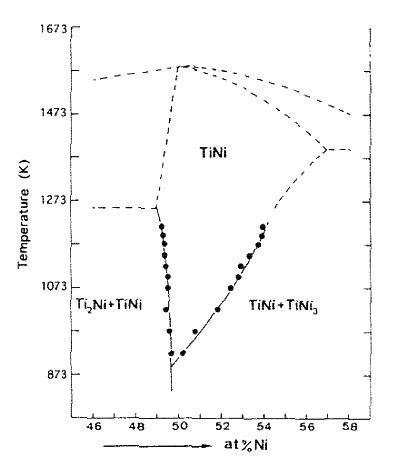
\includegraphics[scale=0.35]{img/DiagramaNiTi.jpg}
					%\caption*{Diagrama de fases de NiTi centrado en 50\%.}
					\end{figure}
				\end{column}
				\begin{column}{.49\textwidth}
				A las propiedades ya mencionadas, la aleación $NiTi$ adicionalmente posee:
					\begin{itemize}
						\item Alta vida útil antes de sufrir fatiga
						\item Resistencia a la corrosión
						\item Biocompatible
					\end{itemize}
				\end{column}
			\end{columns}
		\end{frame}
		
	\subsection{Materiales con memoria de forma de alta temperatura}
		\begin{frame}{Materiales con memoria de forma de alta temperatura}
			Las aplicaciones actuales de los SMA están limitadas por debajo de los $100^\circ C$. Los materiales con memoria de forma de alta temperatura, abreviados como \textbf{HTSMA} (del inglés, \textbf{H}igh \textbf{T}emperature \textbf{S}hape \textbf{M}emory \textbf{A}lloys) son aquellos en los cuales la transformación martensítica sucede a $T > 100^\circ C$.
			
			Lo más común a es a $NiTi$ agregarle $Pd$ o $Pt$ en detrimento del $Ni$, pero recientemente se encontró que $Hf$ o $Zr$ en lugar del $Ti$ tienen efectos aún mayores en la temperatura a menor costo relativo.
		\end{frame}
		
	\subsection{Objetivo}
		\begin{frame}{Objetivo}
			El objetivo del presente estudio es, sabiendo que la aleación $NiTi$ presenta el efecto de memoria de forma, agregarle $Zr$ en detrimento del $Ti$ con la expectativa que las temperaturas en las cuales sucede el efecto de memoria de forma sean superiores a los 100$^\circ C$. El material se estudia en forma de láminas delgadas depositadas mediante magnetrón sputtering.
		\end{frame}
		
	\subsection{Cristalización}
		\begin{frame}{Cristalización}
			\begin{figure}
				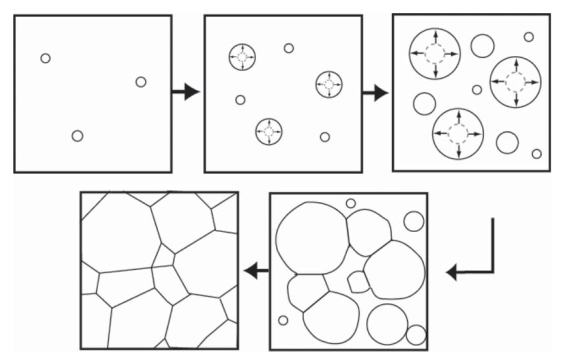
\includegraphics[scale=0.35]{img/cristalization.png}
				\caption*{Esquema de nucleación y crecimiento.}
			\end{figure}
		\end{frame}
		
		\begin{frame}{Ecuación de Johnson-Mehl}
			\begin{columns}[T]	
				\begin{column}{.4\textwidth}
					\begin{figure}
						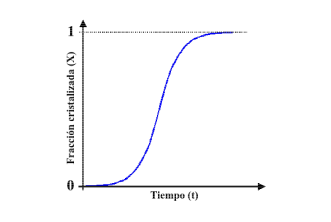
\includegraphics[scale=0.3]{img/cristalization_vs_tiempo.png}
						\caption*{Esquema cristalización en función del tiempo}
					\end{figure}
				\end{column}
				\begin{column}{.59\textwidth}
					Asumiendo velocidad de nucleación constante $I$ y velocidad de transformacion $\Gamma$ isótropica, en un comienzo la transformación estará gobernada por $X_e(t) = \frac{\pi}{3}\Gamma^3 I t^4$.
					
					A tiempos grandes, la función debe saturar en 1, esto se representa mediante la ecuación diferencial $dX = (1 - X)dX_e$, cuya solución es $X(t)=1-e^{-\frac{\pi}{3}V^3 I t^4}$. Esta se conoce como la ecuación de Johnson-Mehl.
				\end{column}
			\end{columns}
		\end{frame}
		\begin{frame}{Modelo de Avrami}
		Ahora cambiamos la hipótesis inicial a que I no es constante, sino que la velocidad de nucleación decaerá a medida que la muestra vaya transformando. Esto es $N(t) = N_0e^{-\nu t}$. Esto genera que para valores cercanos a de t a 0 recuperamos la ecuación de Johnson-Mehl, pero para valores altos, tendremos $X = 1 - exp\left\lbrace -\frac{4}{3} \pi N_0 \nu^3 t^3 \right\rbrace$, que en forma genérica es de la forma $X = 1 - e^{-(kt)^n}$, $k=fe^{-\frac{E_c}{RT}}$, siendo n el coeficiente de Avrami, $f$ el factor de frecuencia y $E_c$ la energía de cristalización.
		\end{frame}
		
		\begin{frame}{Métodos de Kissinger y Augis-Bennet}
			\begin{columns}
				\begin{column}{.49\textwidth}
					Kissinger \\ Es un caso particular del modelo de Avrami con n=1, esto es $X(t) = 1 - e^{-kt}$. Suponiendo que $T(t) = T_0+\alpha t$ como suele ser el caso de un DSC, queda $fe^{-\frac{E_c}{RT}} = \frac{\alpha E_c}{R T_p^2}$ y, simplificando, $ln(\frac{\alpha}{R T_p^2}) = -\frac{E_c}{RT_p} + cte$.
				\end{column}
				\begin{column}{.49\textwidth}
				Augis-Bennet\\
				Considera que el proceso es aproximable por una serie de pasos isotérmicos. Suponiendo que $T(t) = T_0+\alpha t$, queda $k\: t = f\: t\: exp \left\lbrace -\frac{E_c}{R(T_0 + \alpha t)} \right\rbrace$, que permite reescribir el modelo de Avrami como $X = 1-e^{-u^{n}}$. Con este modelo finalmente se obtiene $f^n exp \left\lbrace -\frac{n E_c}{RT_p} \right\rbrace = (\frac{\alpha}{T_p - T_0})^n$  y simplificando $ln(\frac{\alpha}{T_p - T_0}) = -\frac{n E_c}{RT_p} + cte$.
				\end{column}
			\end{columns}
		\end{frame}	
		
		
	\subsection{Transformación martensítica}
		\begin{frame}{Transformación martensítica}
			La causa del efecto de memoria de forma es la transformación martensítica.
			Sus propiedades son
			\begin{itemize}
				\item Transformación de estado sólido
				\item Primer orden
				\item Sin difusión atómica
				\item Desplazamiento de los átomos del orden de 1 \AA
				\item Los átomos mantienen relación con sus vecinos cercanos
			\end{itemize}
		\end{frame}
		
		\begin{frame}
			Usualmente la fase existente a mayor temperatura, llamada fase matriz o austenita, es cúbica, mientras que la fase de menor temperatura, llamada martensita debe tener menor simetría que la fase matriz, esto es, debe ser monoclínica u ortorrómbica. En el caso de $NiTi$ la austenita es la fase B2 y la martensita, la B19'.
			\begin{figure}[H]
			\captionsetup[subfloat]{labelformat=empty}
				\subfloat[Fase B19'.]{
					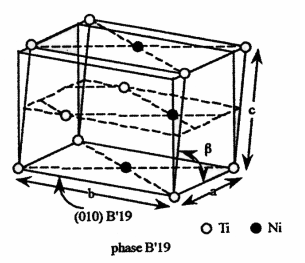
\includegraphics[scale=0.4]{img/B19pPhase.png}
				}
				\subfloat[Fase B2.]{
					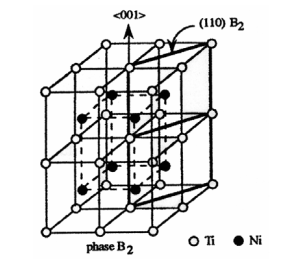
\includegraphics[scale=0.4]{img/B2Phase.png}
				}
			\end{figure}
		\end{frame}

		\begin{frame}{Temperatura de la transformación}
			\begin{columns}[T]
				\begin{column}{.49\textwidth}
					\begin{figure}
						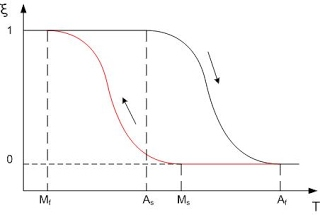
\includegraphics[scale=0.5]{img/Sma_wire.jpeg}
						\caption*{Esquema porcentaje de fases en función de la temperatura.}
					\end{figure}
				\end{column}
				\begin{column}{.49\textwidth}
					\begin{figure}
						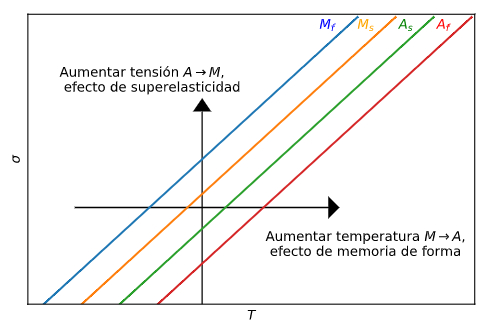
\includegraphics[scale=0.3]{img/TvsStress.png}
						\caption*{Esquema temperaturas de transformación en función de la tensión.}					
					\end{figure}
				\end{column}
			\end{columns}
		\end{frame}
		
		\begin{frame}
			\begin{figure}
				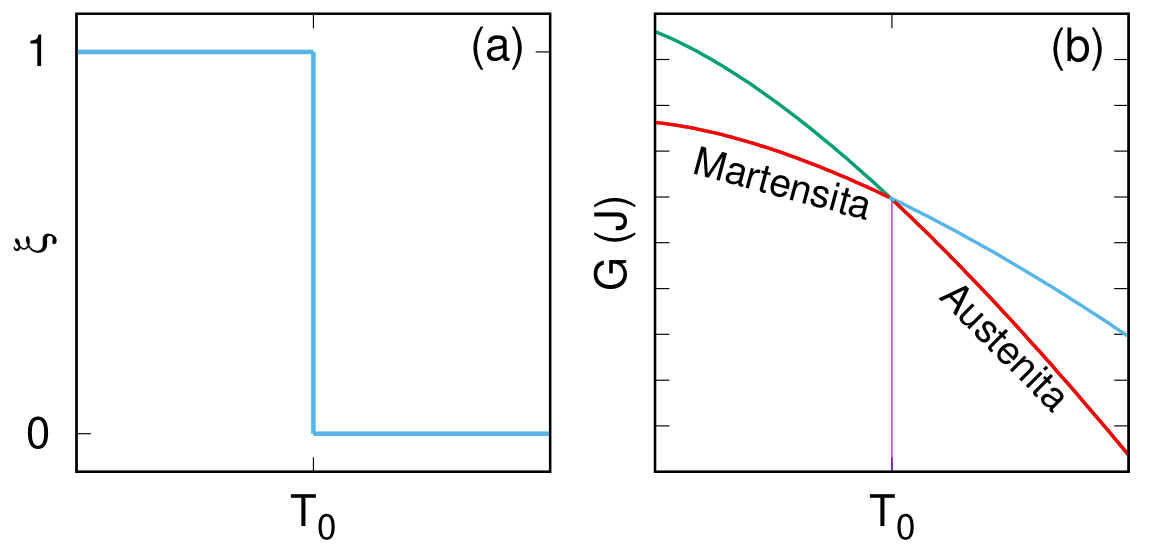
\includegraphics[scale=0.25]{img/GibbsIdealCase.png}
				\caption*{Si la transformación sucediera a la temperatura de equilibrio termodinámico.}		
			\end{figure}
		\end{frame}
		
		\begin{frame}
			\begin{figure}
				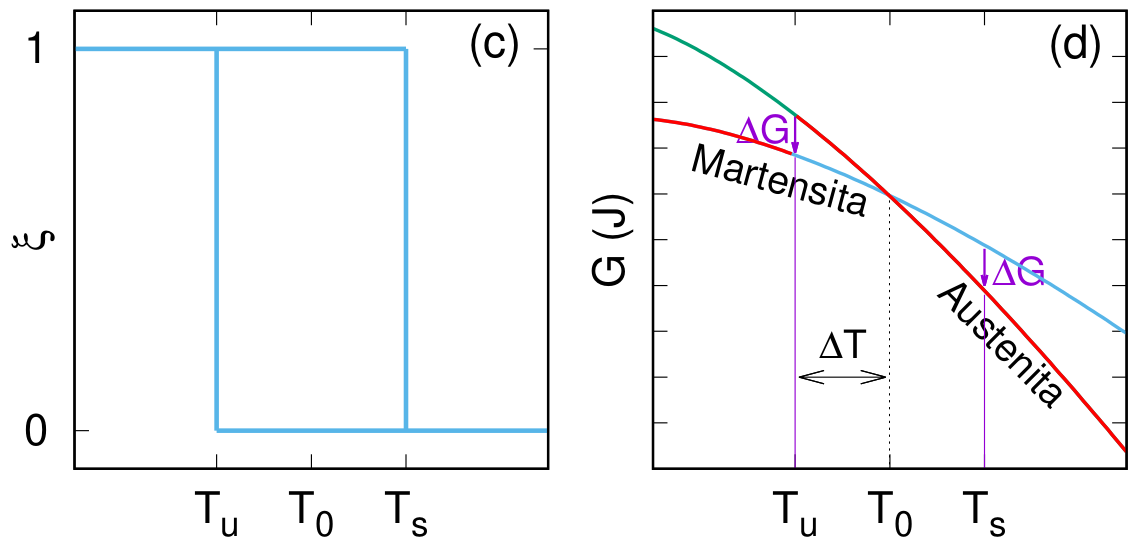
\includegraphics[scale=0.25]{img/GibbsWithFriction.png}
				\caption*{Si sólo hubiera trabajo de fricción.}
			\end{figure}
		\end{frame}

		\begin{frame}
			\begin{figure}
				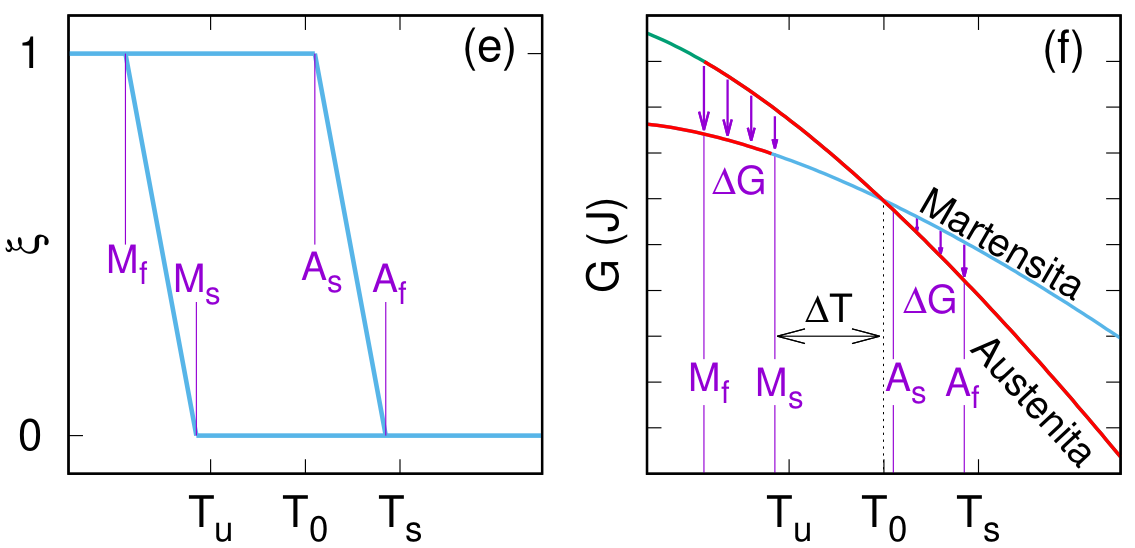
\includegraphics[scale=0.25]{img/GibbsElasticEnergy.png}
				\caption*{Si hubiera tanto trabajo de fricción como trabajo elástico}
			\end{figure}
		\end{frame}


\section{Técnicas experimentales}

	\subsection{Deposición por magnetrón sputtering}
		\begin{frame}{Deposición por magnetrón sputtering}
			\begin{columns}[T]
				\begin{column}{.4\textwidth}
					\begin{figure}[H]
					\centering
					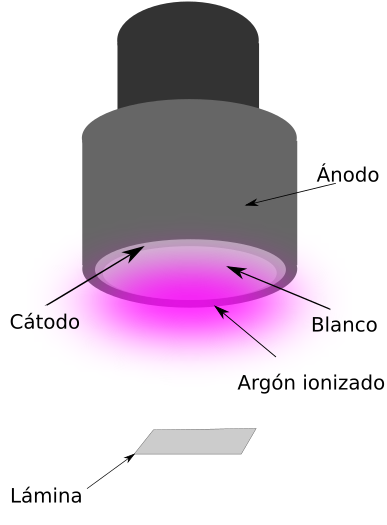
\includegraphics[scale=0.25]{img/SchemaDeposition.png}
					%\caption*{Esquema magnetrón sputtering.}
					\end{figure}
				\end{column}
				\begin{column}{.58\textwidth}
					\begin{figure}[H]
					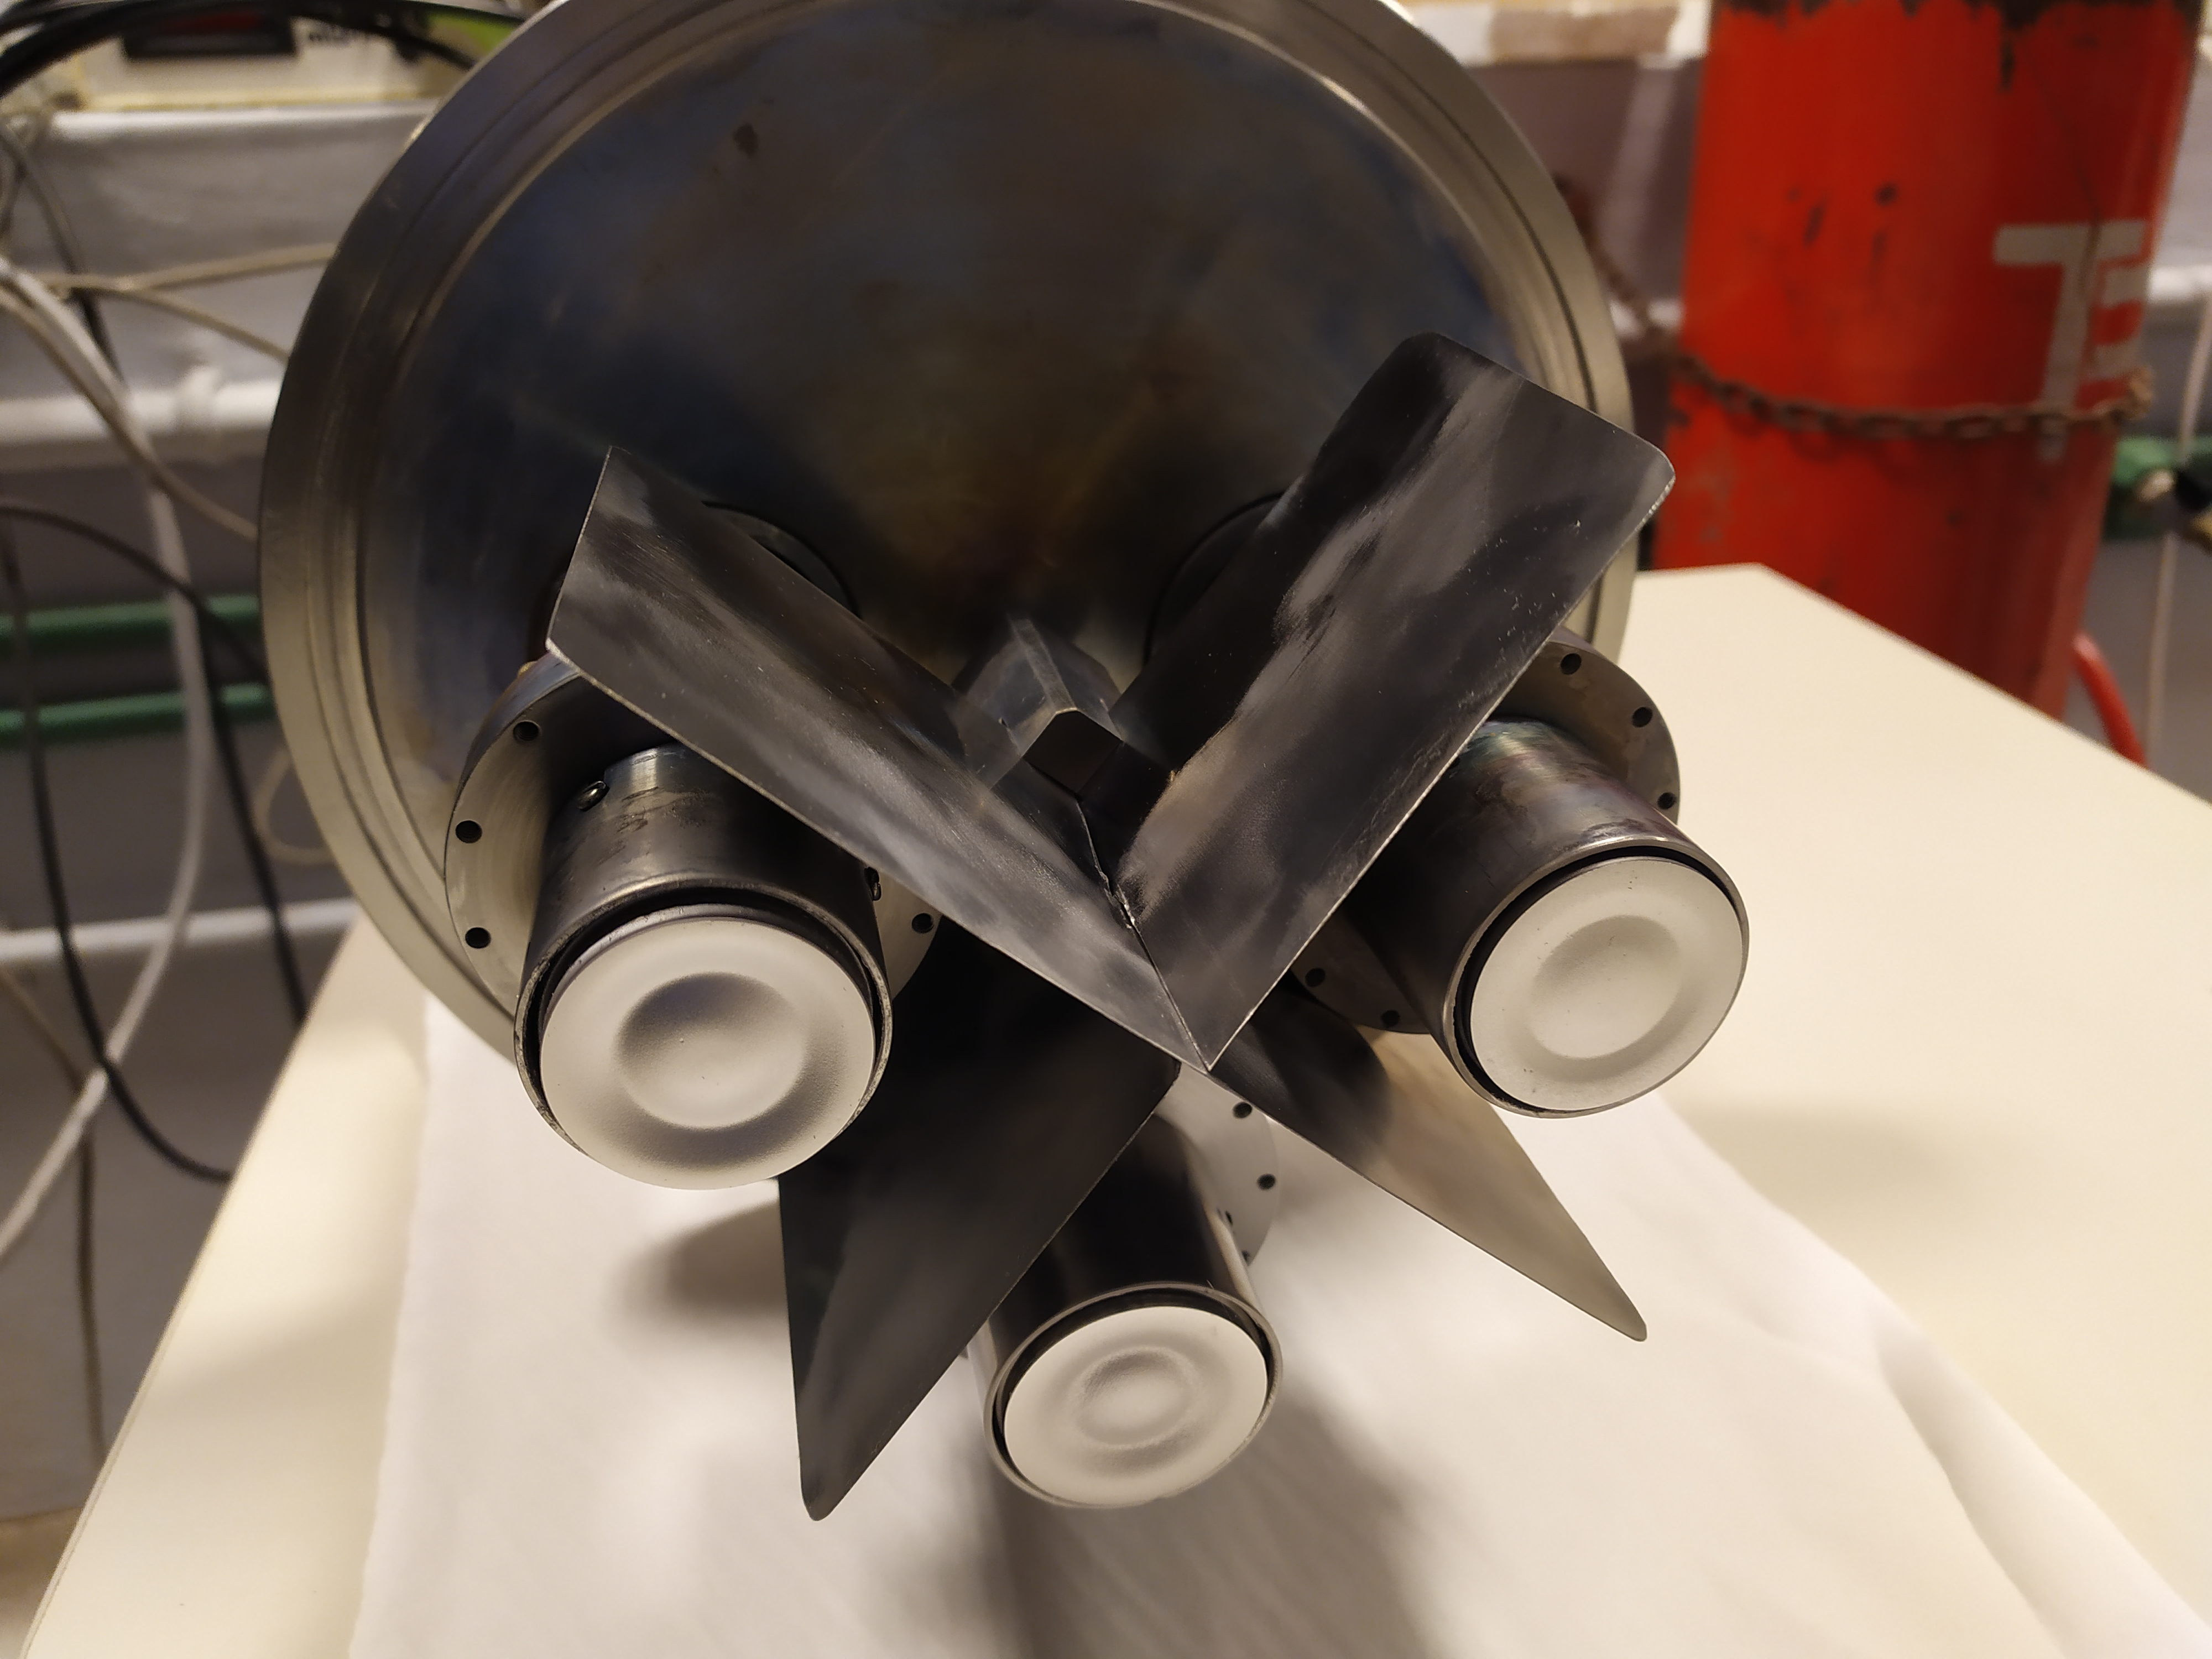
\includegraphics[scale=0.04]{img/magnetrones.jpg}
					\caption*{Magnetrones empleados.}
					\end{figure}
				\end{column}
			\end{columns}
		\end{frame}
		
		\begin{frame}{Cámara empleada}
			\begin{columns}[T]
				\begin{column}{.49\textwidth}
					\begin{figure}[H]
					\centering
					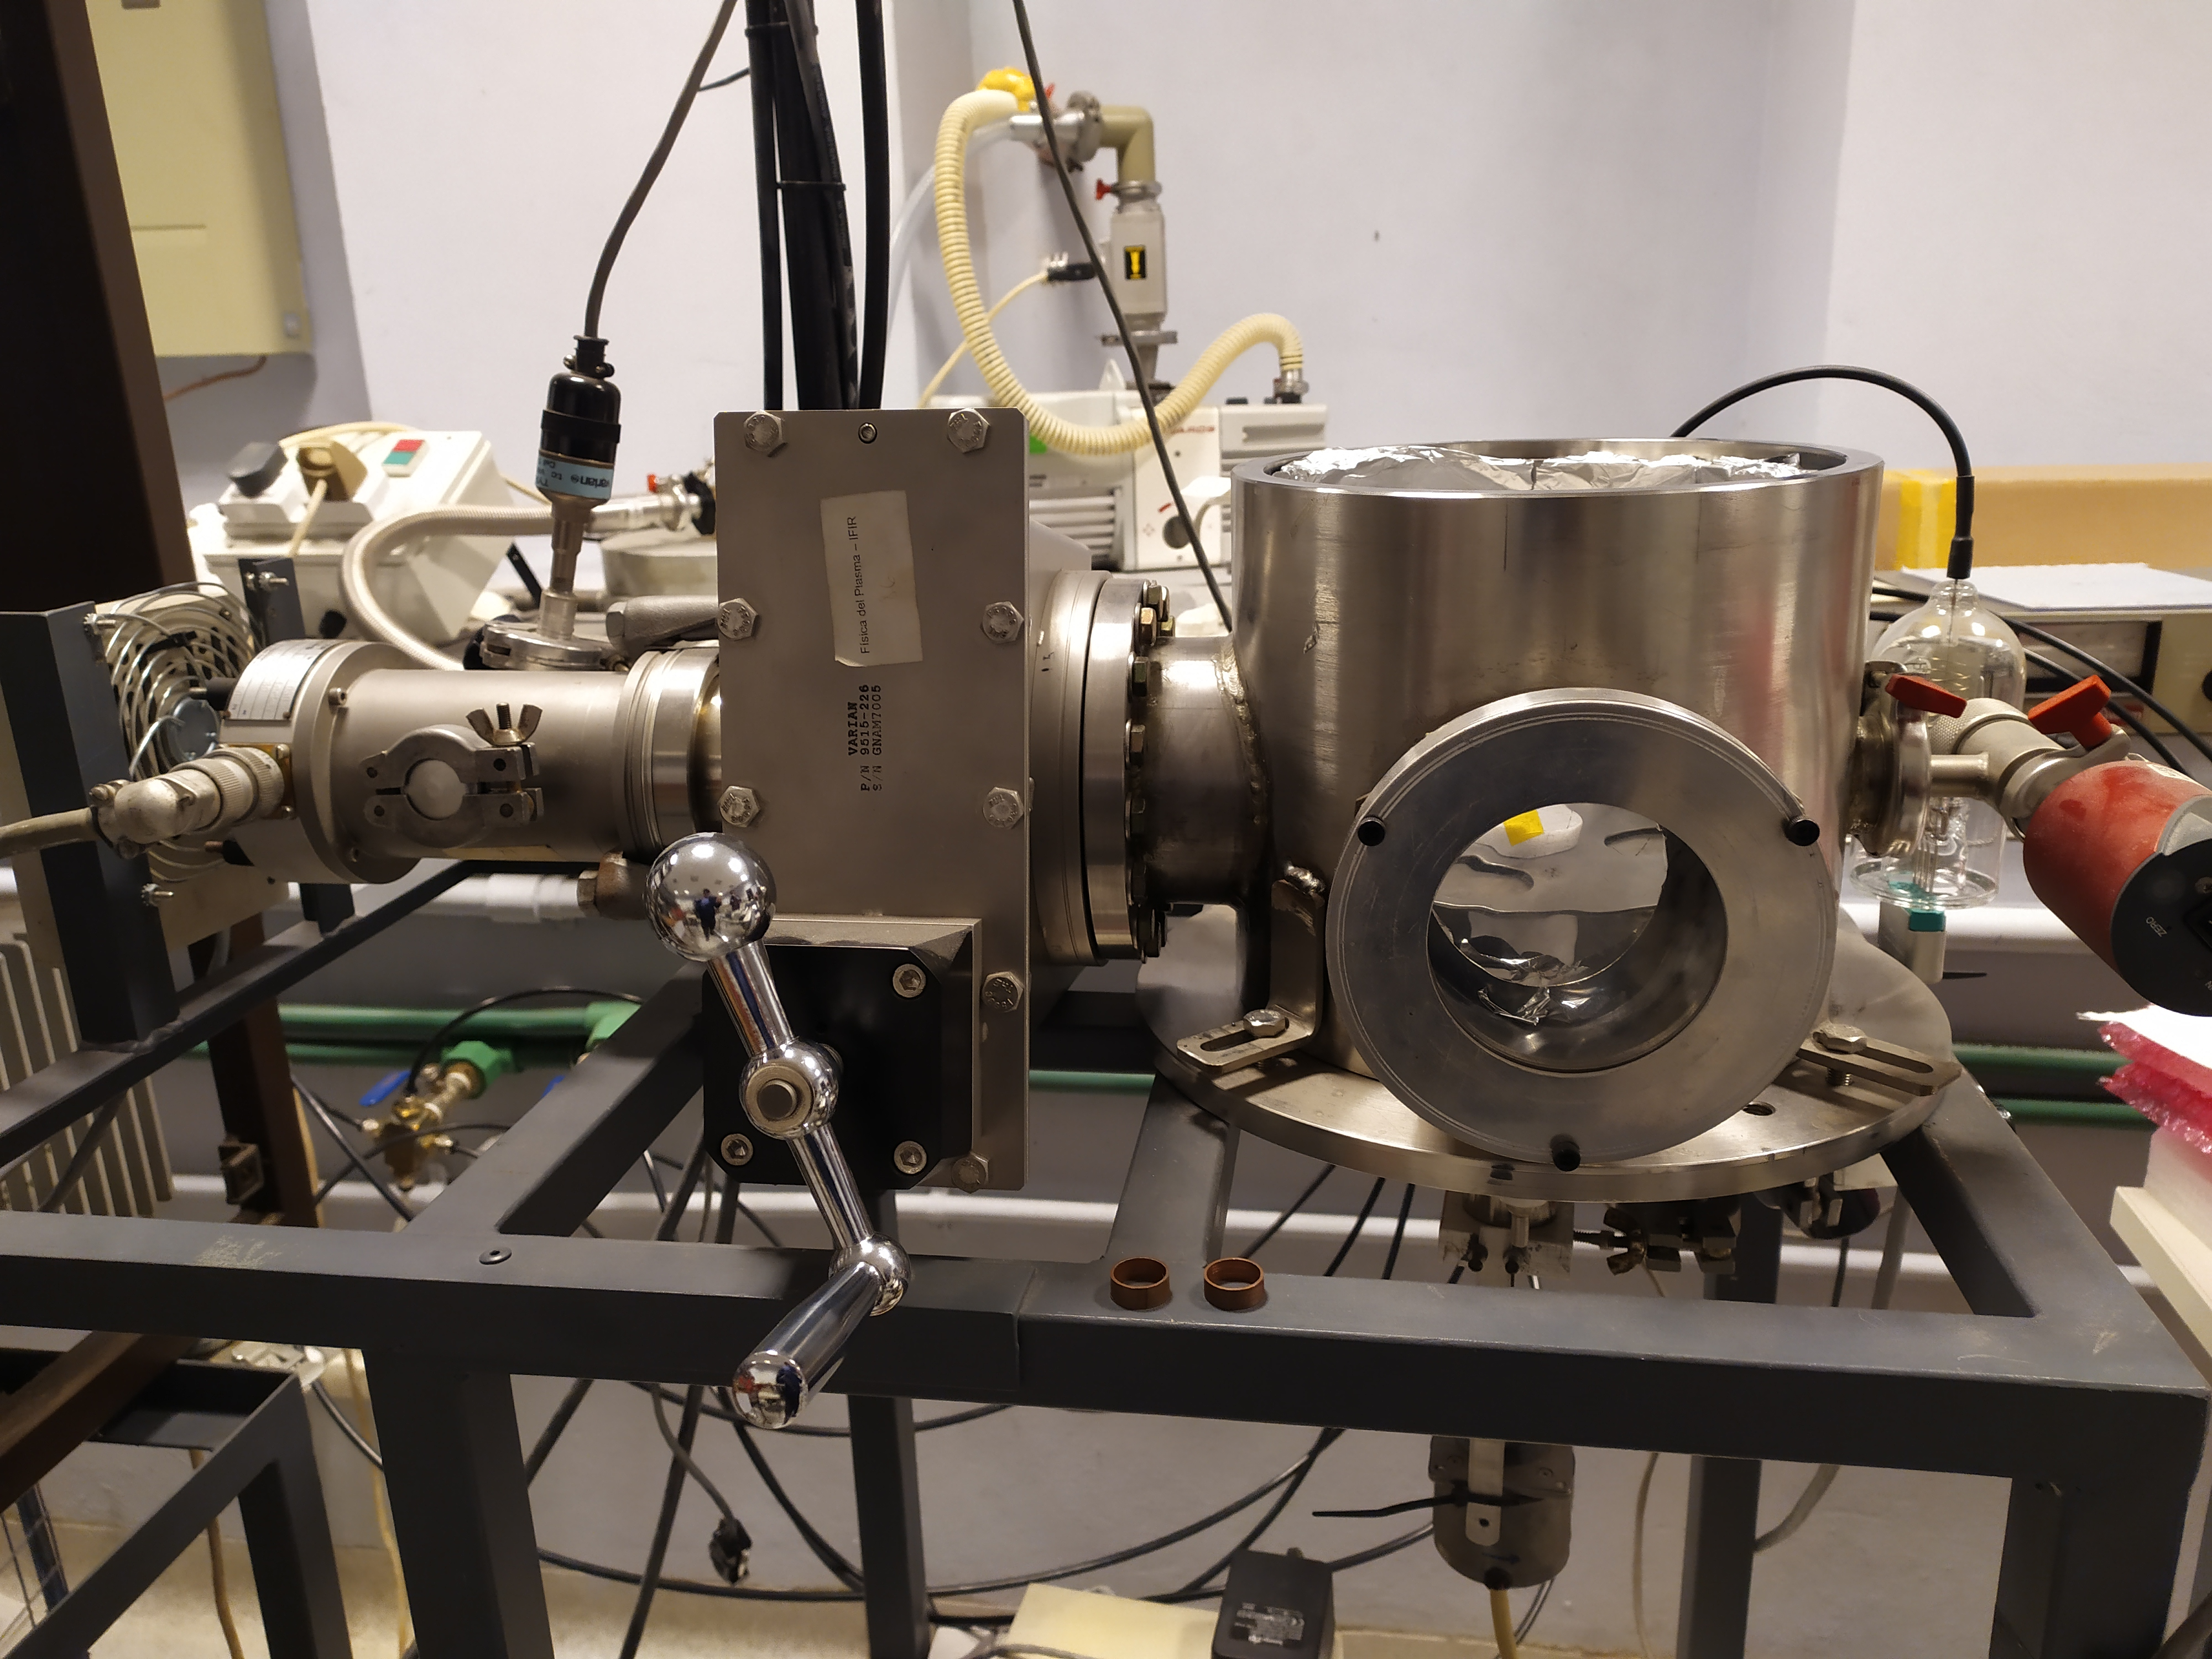
\includegraphics[scale=0.04]{img/camara.jpg}
					\caption*{Exterior de la cámara.}
					\end{figure}
				\end{column}
				\begin{column}{.49\textwidth}
					\begin{figure}[H]
					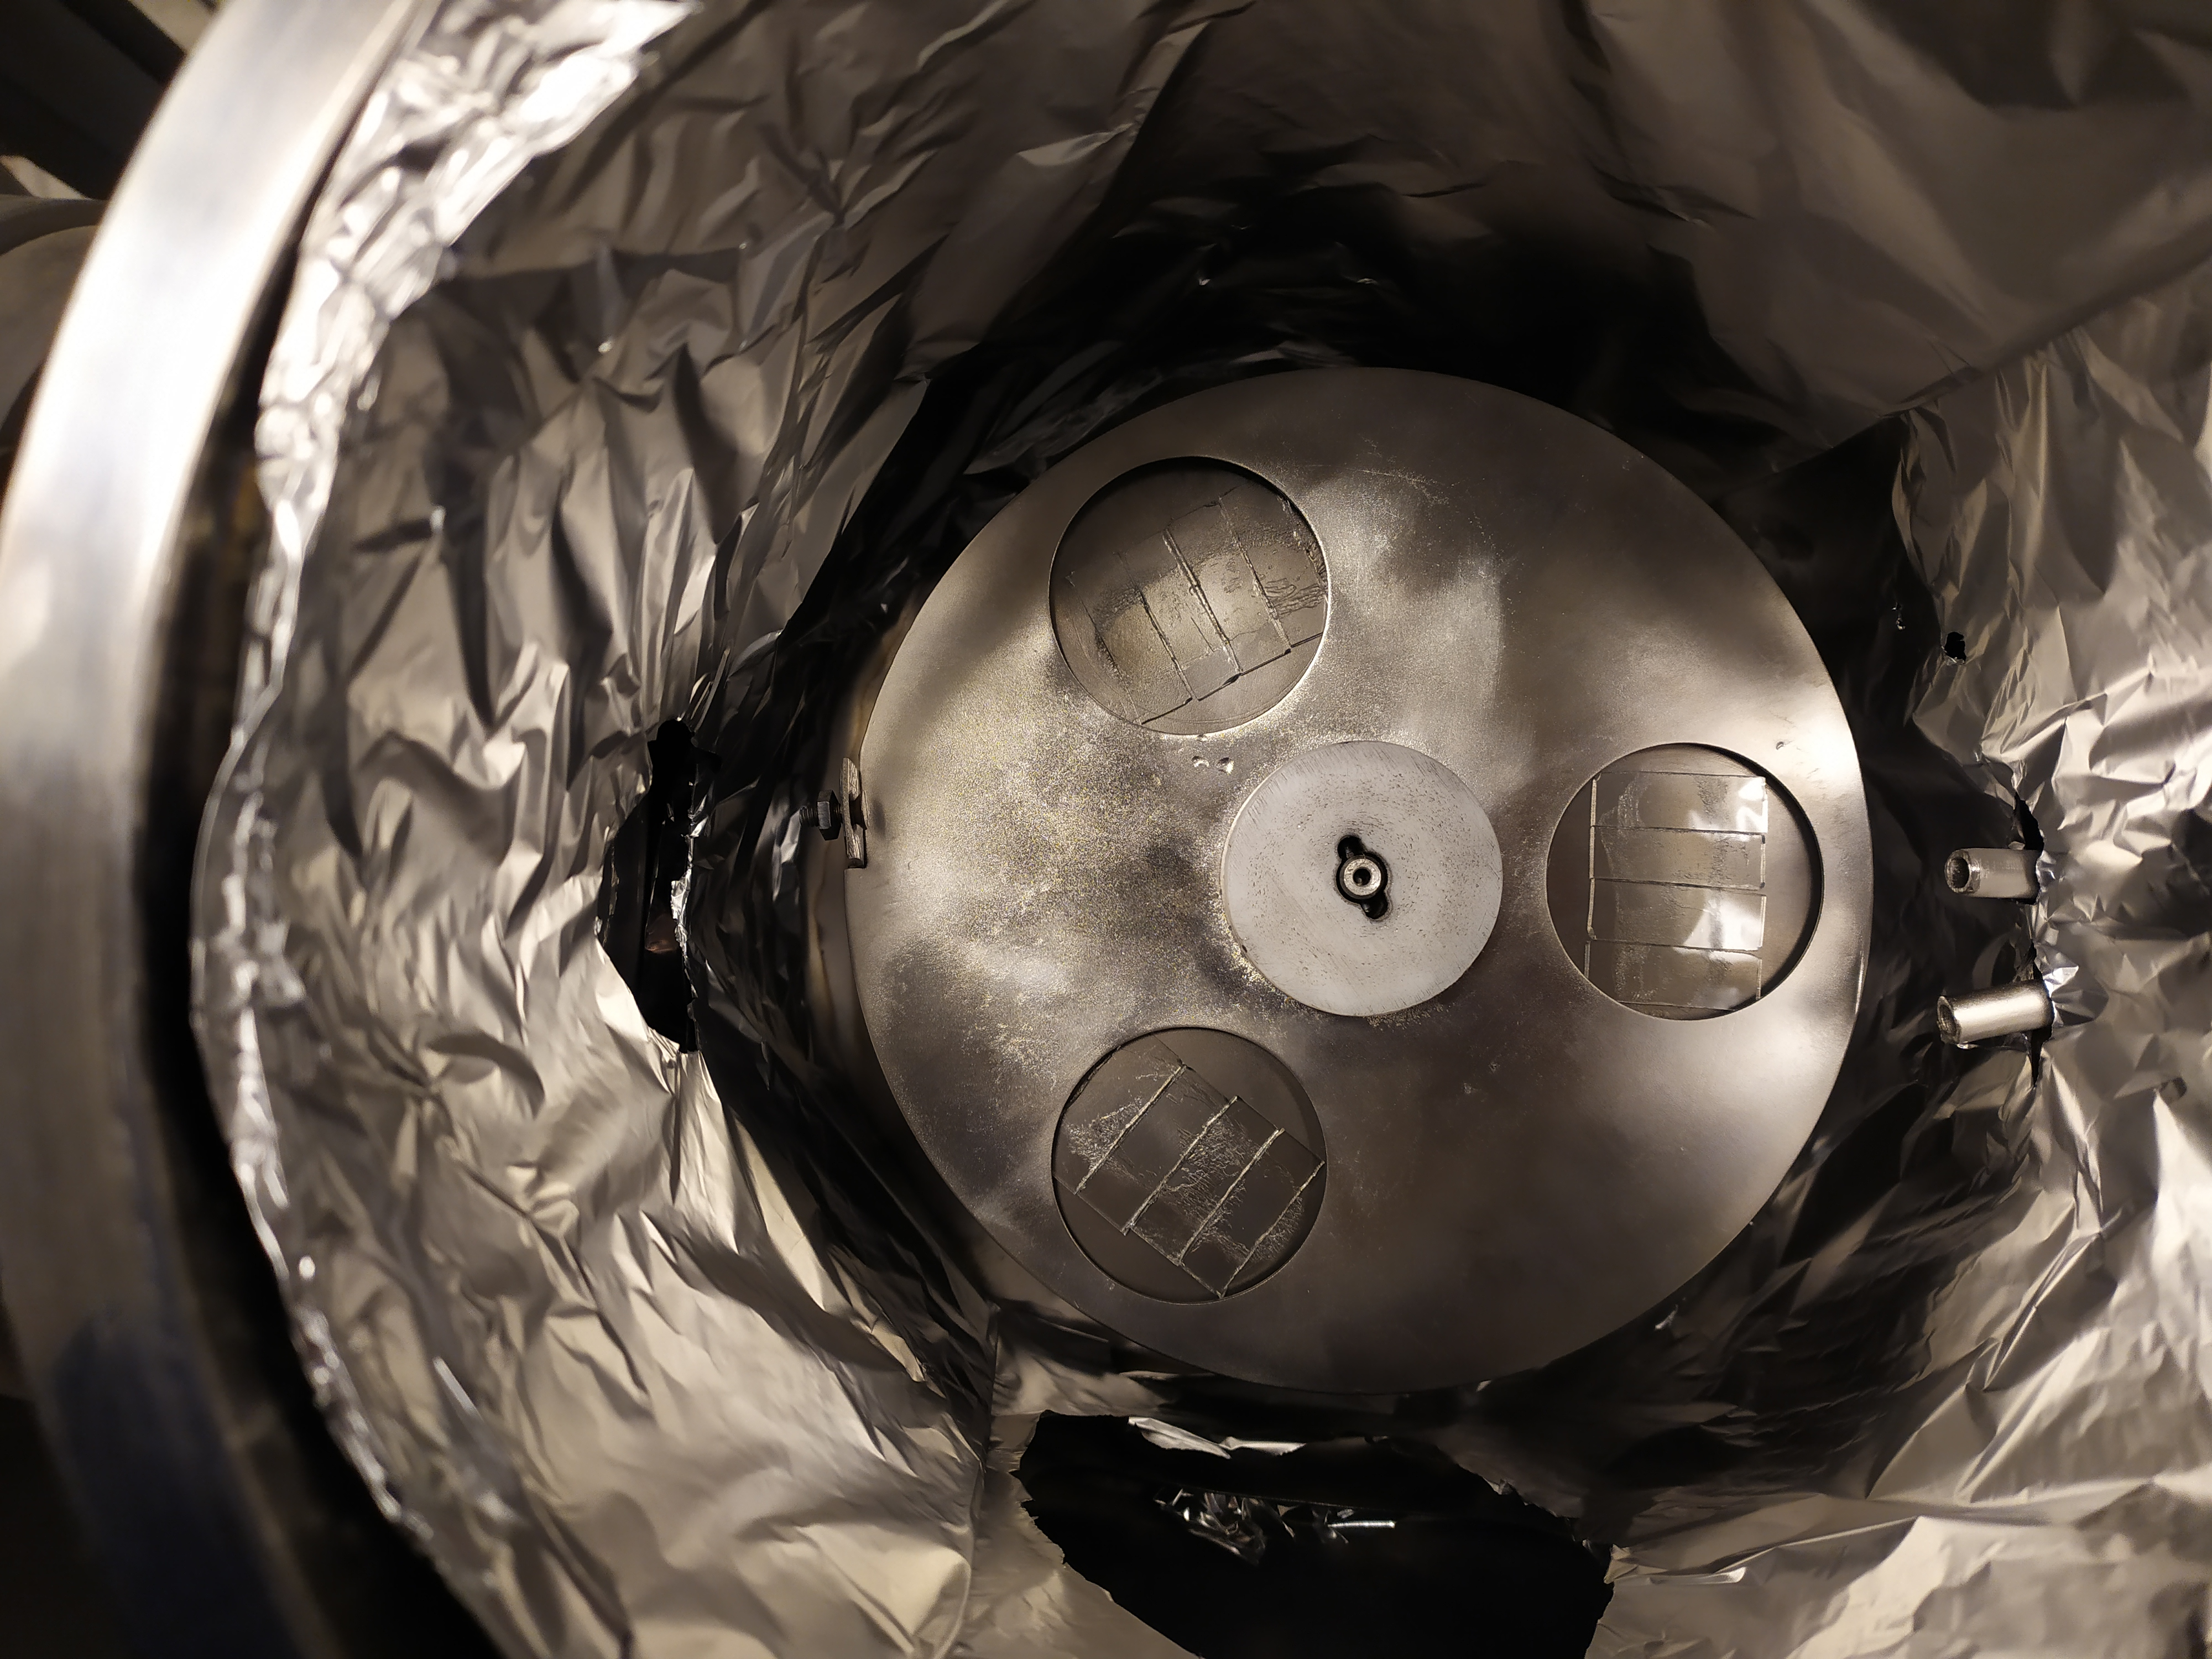
\includegraphics[scale=0.04]{img/muestras.jpg}
					\caption*{Interior de la cámara.}					
					\end{figure}
				\end{column}
			\end{columns}
		\end{frame}
	
	\subsection{Microscopía electrónica de barrido}
		\begin{frame}{Microscopía electrónica de barrido}
			\begin{figure}[H]
				\centering
				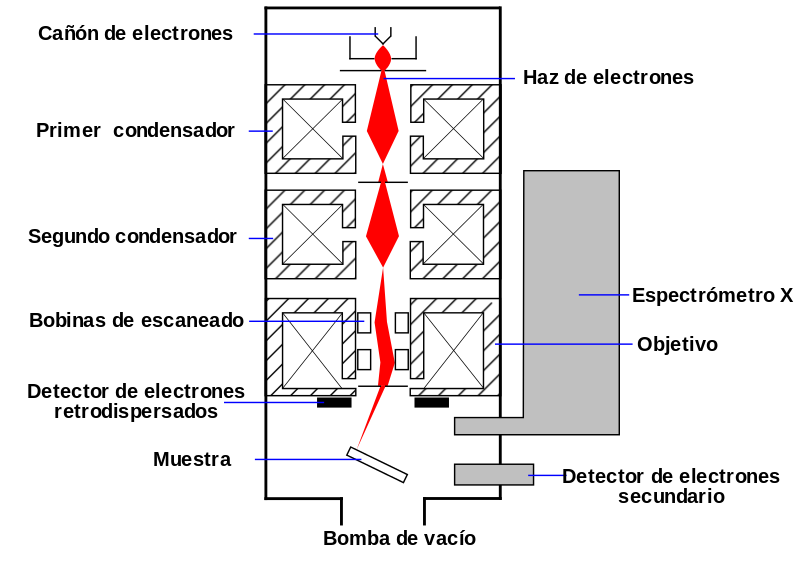
\includegraphics[scale=0.25]{img/SEM.png}
				\caption*{Esquema microscopio electrónico de barrido.}
			\end{figure}
		\end{frame}
		
	\subsection{Tratamientos térmicos}
		\begin{frame}{Tratamientos térmicos}
			\begin{figure}
				\centering
				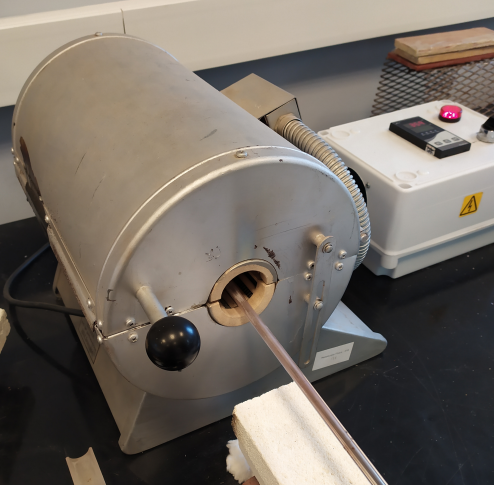
\includegraphics[scale=0.3]{img/hornito.png}
				\caption*{Horno tubular empleado para tratamientos térmicos.}				
			\end{figure}
		\end{frame}
	
	\subsection{Difracción por rayos X}
		\begin{frame}{Difracción por RX}
			\begin{columns}
				\begin{column}{.54\textwidth}
					\begin{figure}[H]
						\centering
						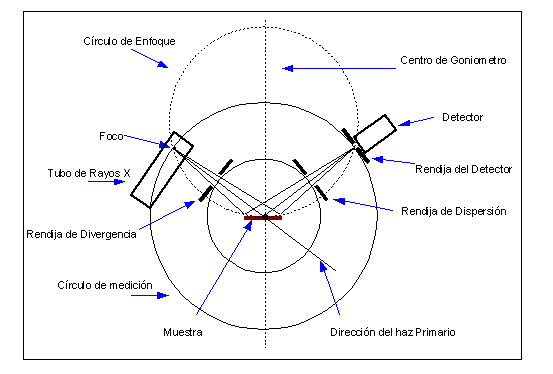
\includegraphics[scale=0.4]{img/gonio.png}
						\caption*{Esquema del dispositivo tipo Bragg-Brentano.}
					\end{figure}
				\end{column}
				\begin{column}{.45\textwidth}
					\begin{figure}[H]
						\centering
						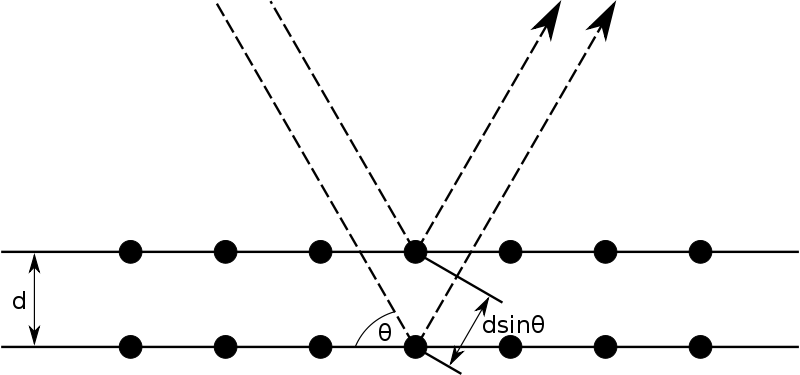
\includegraphics[scale=0.15]{img/Bragg.png}
						\caption*{Reflexión de Bragg en planos atómicos. Los picos de interferencia sucederán cuando  $2 \, d\, {\rm sin} \theta =n \, \lambda \, \,; \, \, n \in \mathbf{N}$}
					\end{figure}
				\end{column}
			\end{columns}
		\end{frame}
	
	\subsection{Microscopía electrónica de transmisión}
		\begin{frame}{Microscopía electrónica de transmisión}
			\begin{figure}[H]
				\centering
				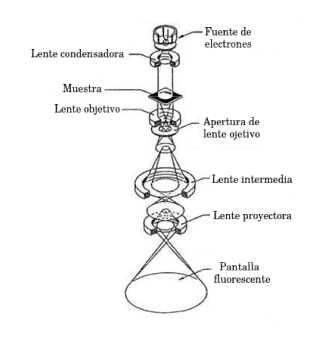
\includegraphics[scale=0.4]{img/TEM.png}
				\caption*{Esquema del tubo de un microscopio electrónico de 							  transmisión.}
			\end{figure}
		\end{frame}

	\subsection{Calorimetría diferencial de barrido}
		\begin{frame}{Calorimetría diferencial de barrido}
			\begin{figure}[H]
				\centering
				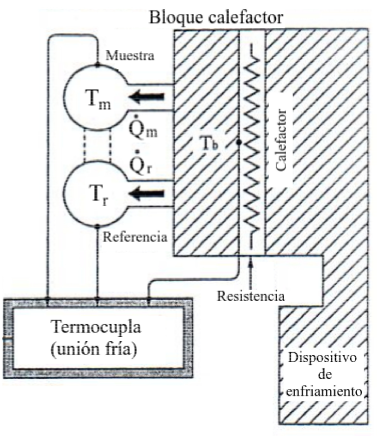
\includegraphics[scale=0.3]{img/DSCscheme.png}
				\caption*{Esquema del DSC empleado.}
			\end{figure}
		\end{frame}

	\subsection{Resistividad por el método de cuatro puntas}
		\begin{frame}{Resistividad por el método de cuatro puntas}
			\begin{columns}
				\begin{column}{.49\textwidth}
					\begin{figure}[H]
						\centering
						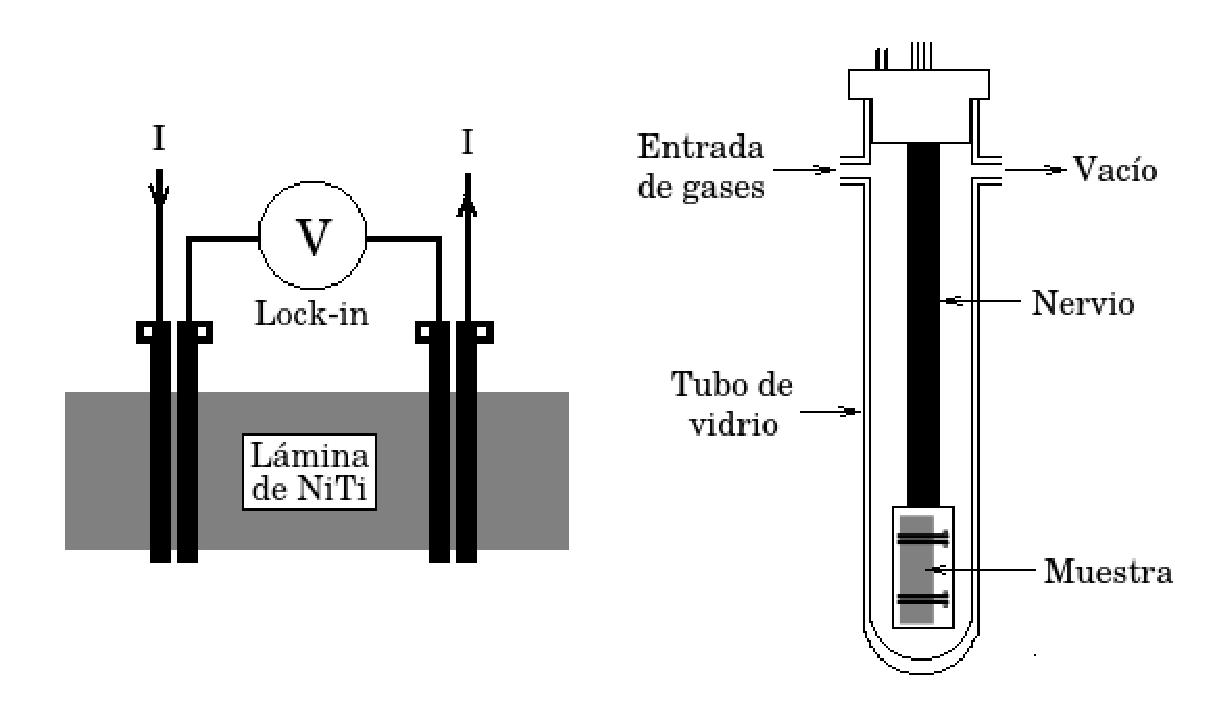
\includegraphics[scale=0.3]{img/resistividad.eps}
						\caption*{Esquema del sistema empleado para el método de 								 resistividad por cuatro puntas.}
					\end{figure}
				\end{column}
				\begin{column}{.49\textwidth}
					\begin{figure}[H]
						\centering
						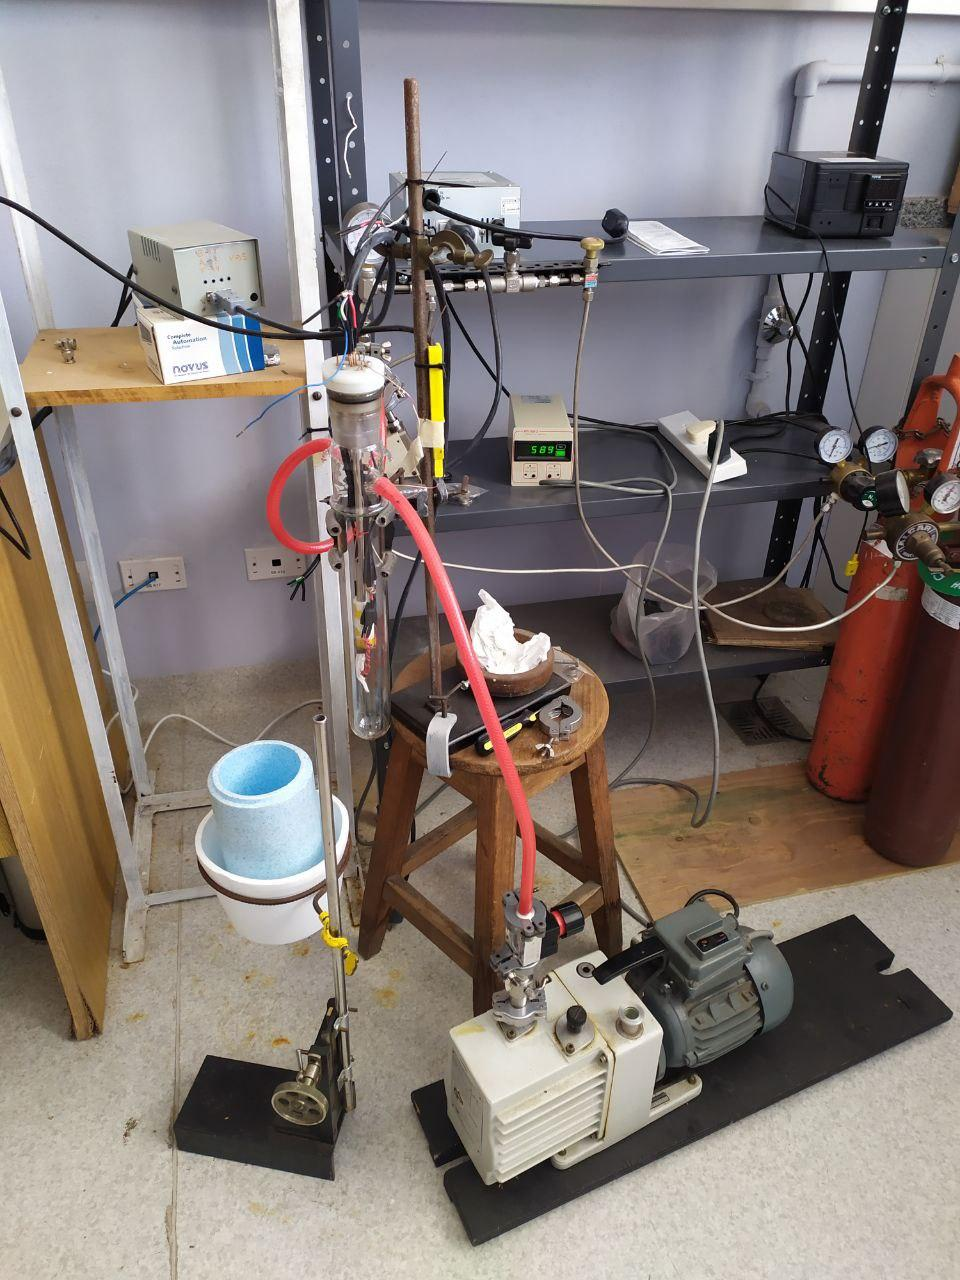
\includegraphics[scale=0.1]{img/resistividad.jpg}
						\caption*{Resistividad por cuatro puntas.}
					\end{figure}
				\end{column}
			\end{columns}
		\end{frame}
	
\section{Resultados obtenidos y discusión}
	\subsection{Deposición de las láminas}
		\begin{frame}
			\begin{figure}
				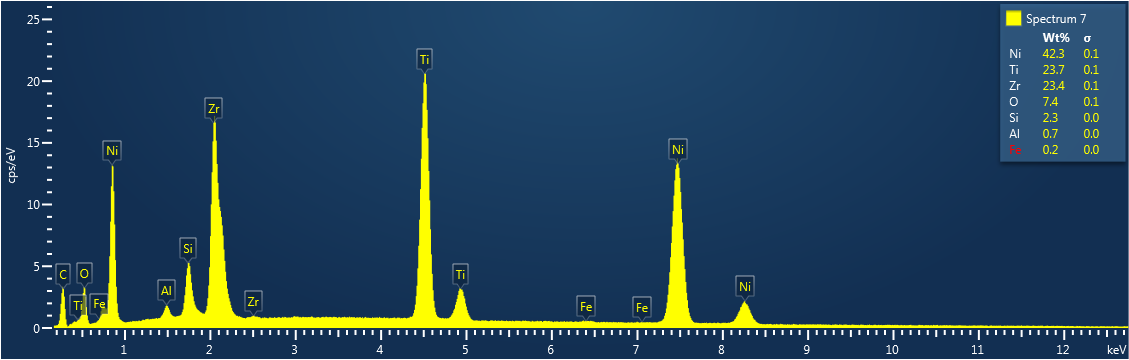
\includegraphics[scale=0.25]{img/SEMAllElements.png}
				\caption*{Resultados de una medición con SEM sin filtrar elementos.}
			\end{figure}
			\begin{table}[H]
				\centering
				\begin{tabular}{c|c|c|}
				\cline{2-3}
				\multicolumn{1}{l|}{} & Primera Deposición & Segunda Deposición \\ \hline
				\multicolumn{1}{|c|}{Ti{[}\%at{]}} & 30,8 $\pm$ 0,6 & 33,2 $\pm$ 0,5 \\ \hline
				\multicolumn{1}{|c|}{Ni{[}\%at{]}} & 50,4 $\pm$ 0,2 & 46 $\pm$ 1 \\ \hline
				\multicolumn{1}{|c|}{Zr{[}\%at{]}} & 18,9 $\pm$ 0,5 & 20,8 $\pm$ 0,4 \\ \hline
				\end{tabular}
				\caption*{Composición determinada para ambas deposiciones.}
				\label{compositionAvg}
			\end{table}
		\end{frame}

	\subsection{Energía de activación}
		\begin{frame}{Energía de activación de la cristalización}
			\begin{figure}
				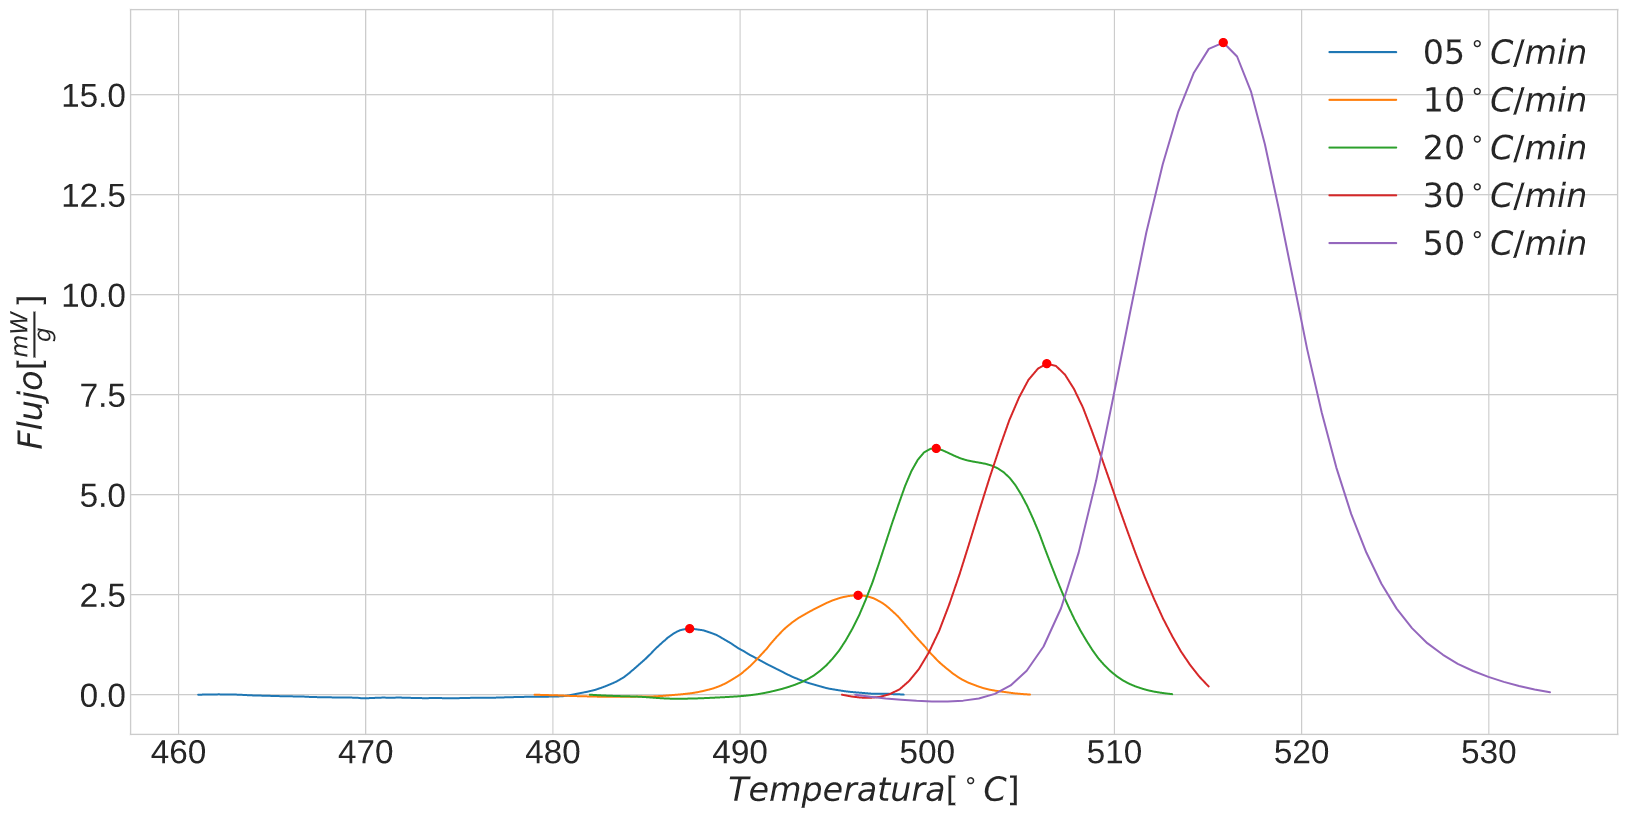
\includegraphics[scale=0.15]{img/DSCPeaks.png}
				\caption*{Flujo de calores a distintas velocidades de calentamiento.}
			\end{figure}
		\end{frame}
		
		\begin{frame}
			\begin{columns}
				\begin{column}{.49\textwidth}
					\begin{figure}
						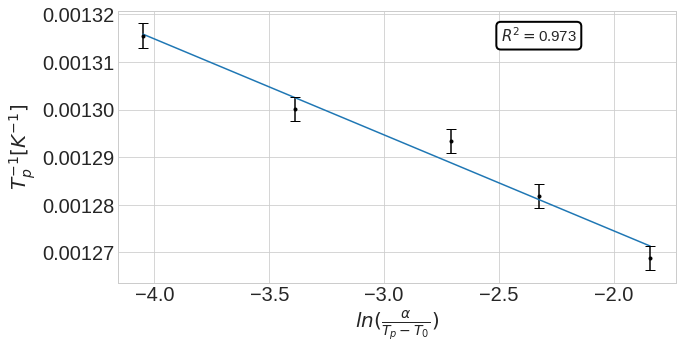
\includegraphics[scale=0.2]{img/Augis_bennet.png}
						\caption*{Regresión por el método de Augis-Bennet. $E_c = 410 \pm 30$ kJ}
					\end{figure}
				\end{column}
				\begin{column}{.49\textwidth}
					\begin{figure}
						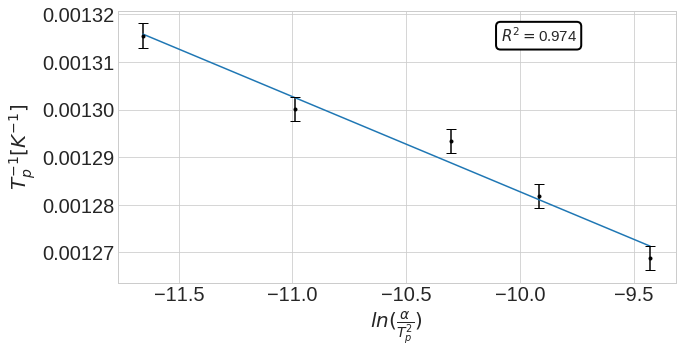
\includegraphics[scale=0.2]{img/Kissinger.png}
						\caption*{Regresión por el método de Kissinger. $E_c = 420 \pm 30$ kJ}				
					\end{figure}
				\end{column}
			\end{columns}
		\end{frame}
		
		\begin{frame}
			\begin{table}[H]
				\centering
				\begin{tabular}{|c|c|c|}
					\hline
					Composición & \begin{tabular}[c]{@{}c@{}}Energía de \\ activacion {[}kJ/mol{]}\end{tabular} & Método \\ \hline
					$Ni_{48,89}Ti_{40,50}Zr_{10,61}$ & 417,2  & composición en cinta\\ \hline
					$Ni_{48,71}Ti_{35,59}Zr_{15,70}$ & 432,9 & composición en cinta\\ \hline
					$Ni_{48,25}Ti_{31,26}Zr_{20,49}$ & 482,4 & composición en cinta\\ \hline
					$Ni_{47,95}Ti_{26,72}Zr_{25,33}$ & 465,8 & composición en cinta\\ \hline
					$Ni_{49,40}Ti_{19,96}Zr_{30,64}$ & 445,7 & composición en cinta\\ \hline
					$Ni_{49,6}Ti_{30,9}Zr_{19,5}$ & 449 $\pm$ 5 & melt spinning\\ \hline
				\end{tabular}
				\caption*{Valores reportados por Xiaoyang Yi et al para la energía de activación para distintas composiciones en cinta.}
				\label{XiaoyangYiValues}
			\end{table}

%Por otra parte, Malvasio en 2017 \citep{Malvasio}, en láminas delgadas obtenidas por deposición mediante magnetrón sputtering en la aleación binaria ($Ni_{54,2}Ti_{45,8}$), obtuvo una energía de activación de $E_c = 300 \pm 30 kJ/mol$ tanto por el método de Kissinger como por el método de Augis-Bennet.
%
%En el presente trabajo se determinó la energía de activación de láminas delgadas de $NiTiZr$ producidas por magnetrón sputtering para la composición rica en $Ni$ ($Ni_{50,4}Ti_{30,8}Zr_{18,9}$) y se obtuvieron valores de $E_c = 420 \pm 30$ kJ por el método de Kissinger y de $E_c = 410 \pm 30$ kJ por el método de Augis-Bennet. Si bien estos valores son levemente inferiores a los determinados por Xiaoyang Yi et al., son notoriamente mayores que los obtenidos en la aleación binaria. La leve diferencia entre los valores determinados en este trabajo con los valores obtenidos por Xiaoyang Yi et al. puede ser entendida teniendo en cuenta las diferentes técnicas de producción. Estas diferencias en los valores de la energía de activación causado por los procesos de producción, ya fueron mostrados en la aleación binaria.
	\end{frame}

	\subsection{Pobres en $Ni$}
		\subsubsection{Fases obtenidas}
			\begin{frame}{Difracción por rayos X I}
				\begin{figure}[H]
					\captionsetup[subfloat]{labelformat=empty}
					\subfloat[Muestra a $500 ^\circ C$]{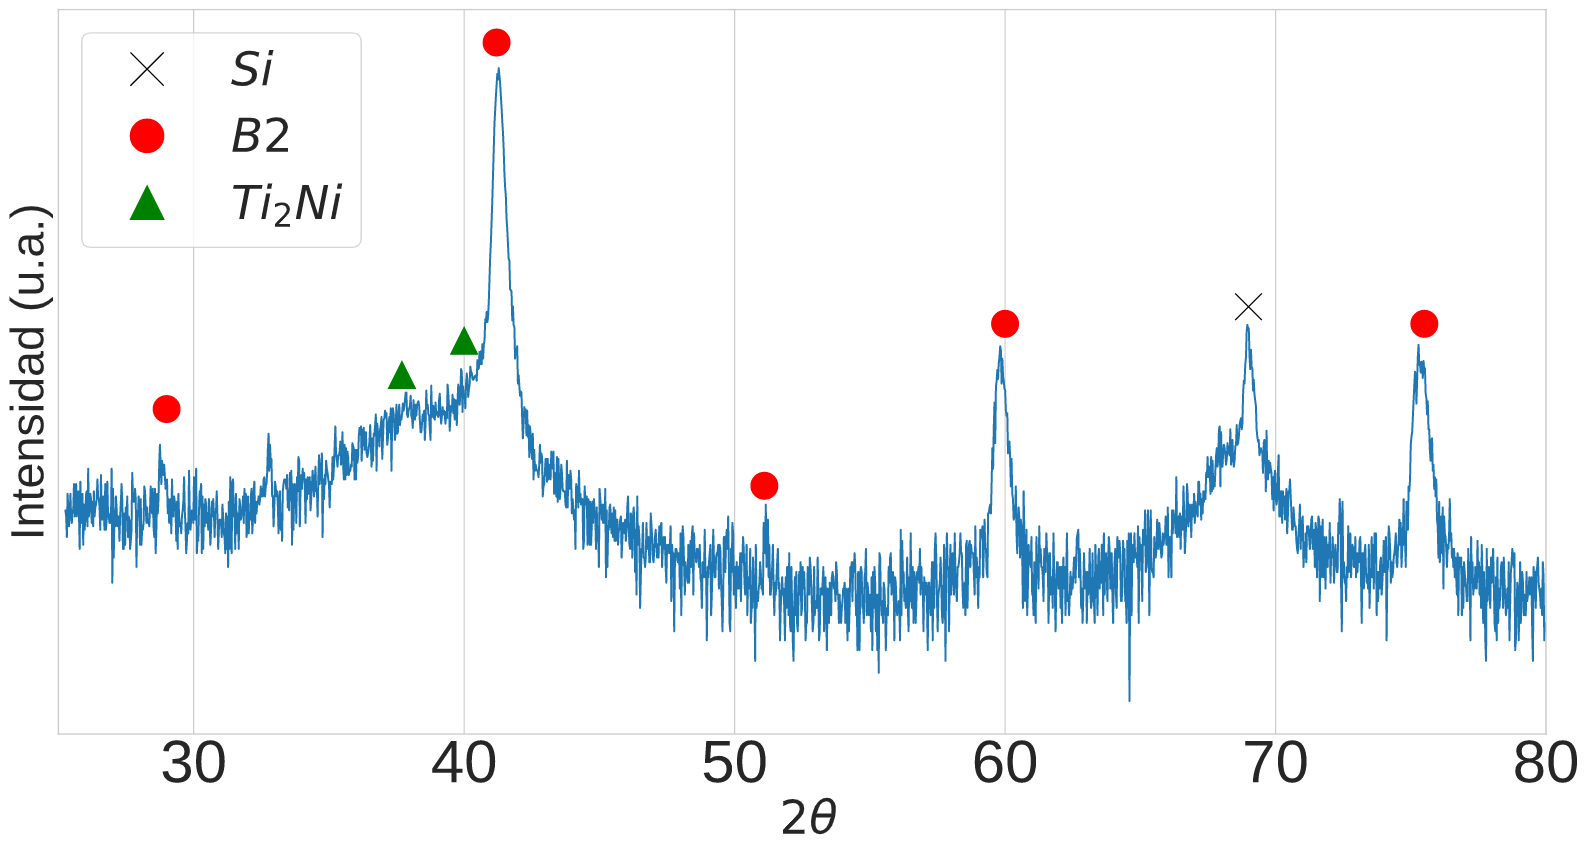
\includegraphics[scale=0.12]{img/RX/NiPoor_500.png}} \qquad
					\subfloat[Muestra a $600 ^\circ C$]{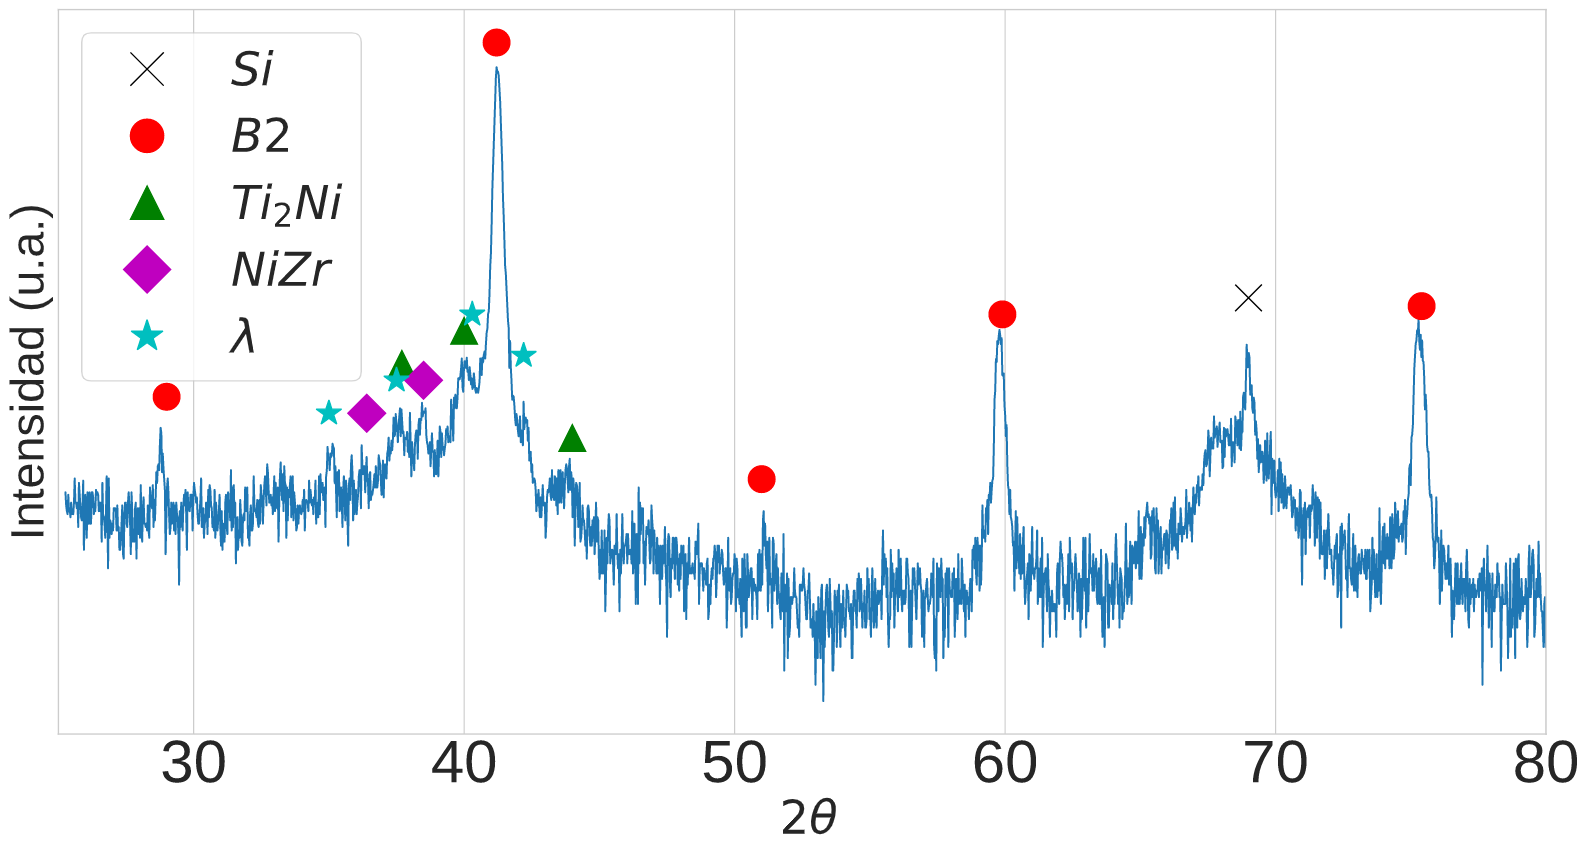
\includegraphics[scale=0.12]{img/RX/NiPoor_600.png}}
					\caption*{Patrones de difracción para las muestras pobres en $Ni$.}
					\label{RXNiPoor}
				\end{figure}		
			\end{frame}
			
			\begin{frame}{Difracción por rayos X II}
				\begin{figure}[H]
					\captionsetup[subfloat]{labelformat=empty}
					\subfloat[Muestra a $700 ^\circ C$]{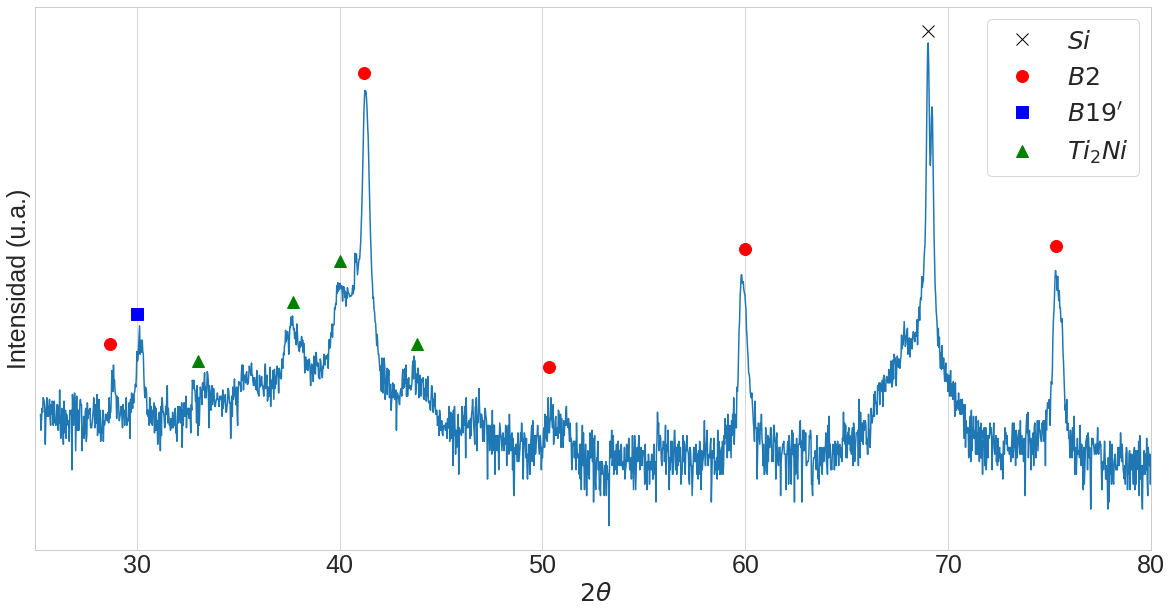
\includegraphics[scale=0.12]{img/RX/NiPoor_700.png}} \qquad
					\subfloat[Muestra a $800 ^\circ C$]{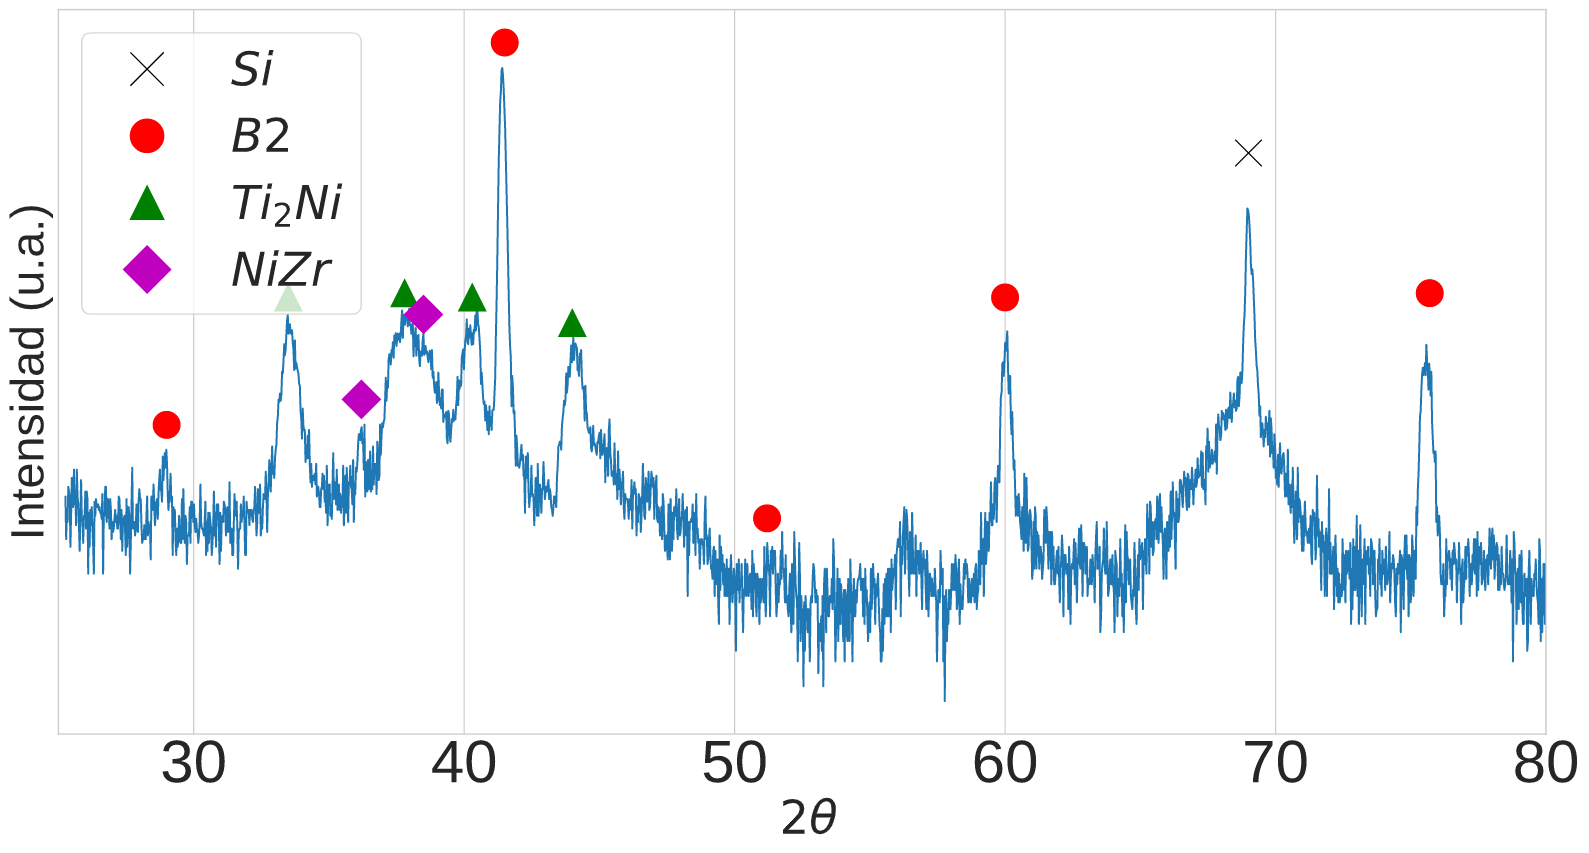
\includegraphics[scale=0.12]{img/RX/NiPoor_800.png}}
					\caption*{Patrones de difracción para las muestras pobres en $Ni$.}
					\label{RXNiPoor}
				\end{figure}		
			\end{frame}
			
			\begin{frame}{Imágenes obtenidas por TEM I}
				\begin{figure}[H]
				\captionsetup[subfloat]{labelformat=empty}
					\centering
					\subfloat[Muestra a $500 ^\circ C$]{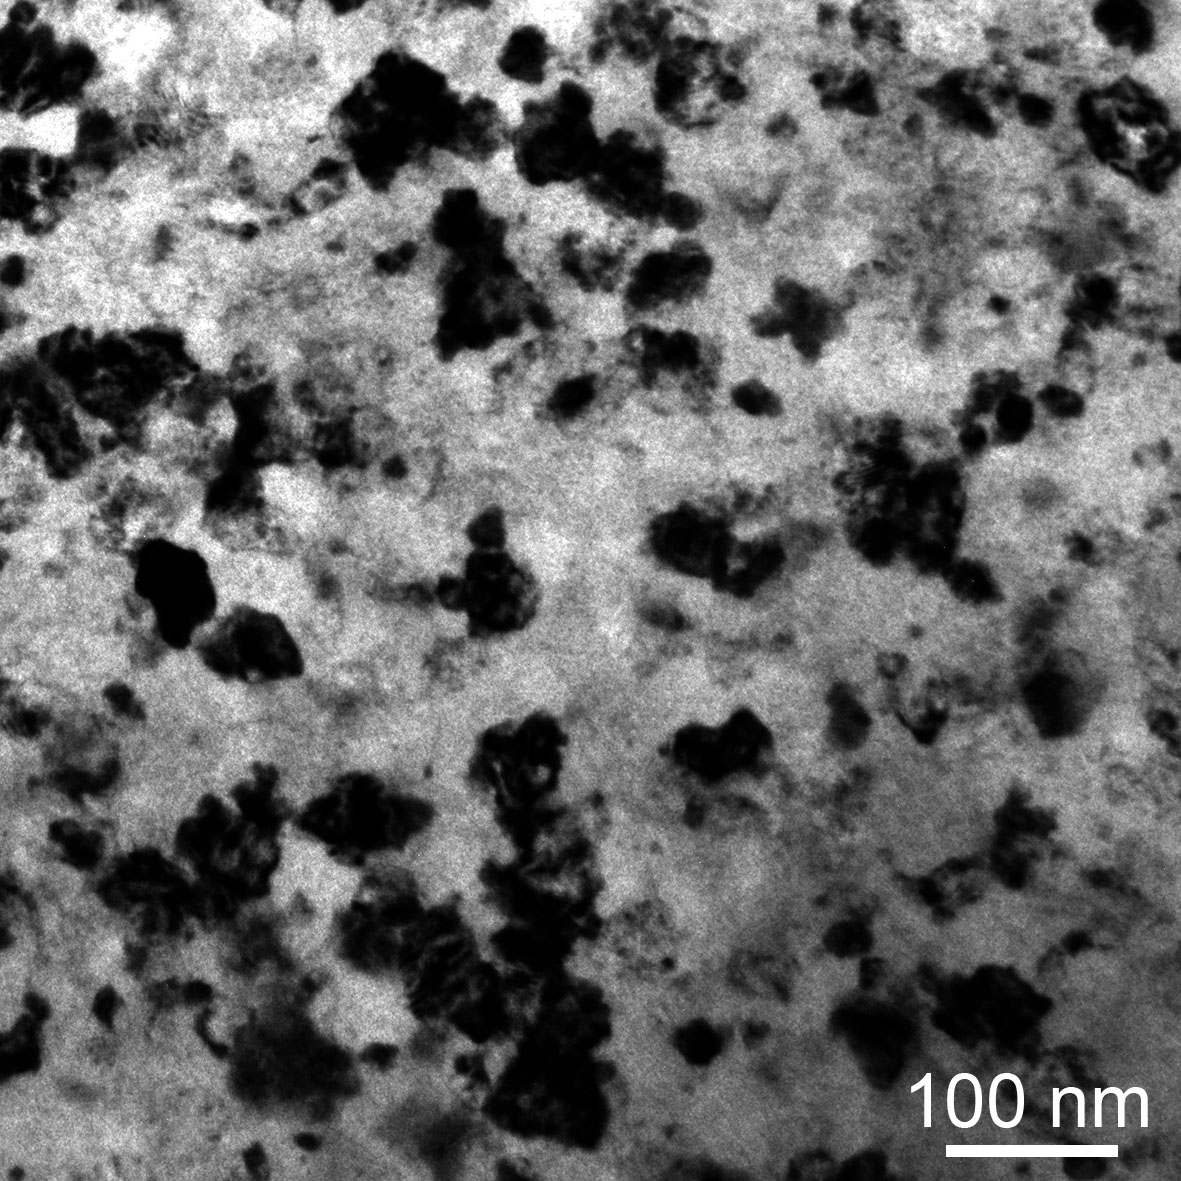
\includegraphics[scale=0.4]{img/TEM/Fig24a.jpg}} \qquad
					\subfloat[Muestra a $600 ^\circ C$]{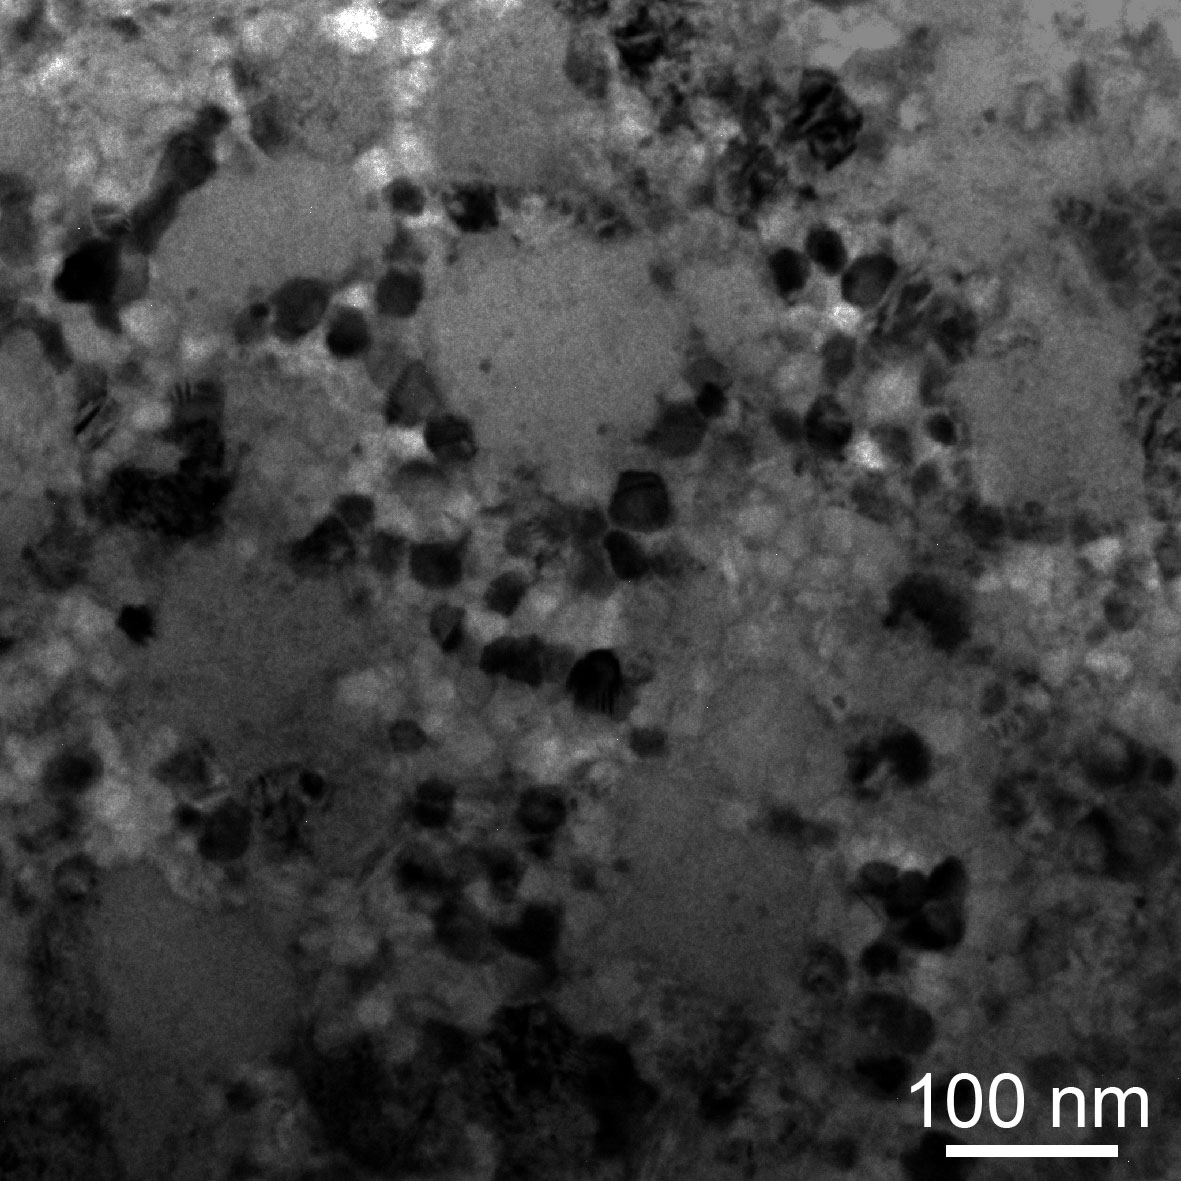
\includegraphics[scale=0.4]{img/TEM/Fig24b.jpg}}
					\caption*{Imágenes de TEM para las muestras pobres en $Ni$.}
				\end{figure}
			\end{frame}
			
			\begin{frame}{Imágenes obtenidas por TEM II}
				\begin{figure}[H]
				\captionsetup[subfloat]{labelformat=empty}
					\centering
					\subfloat[Muestra a $700 ^\circ C$]{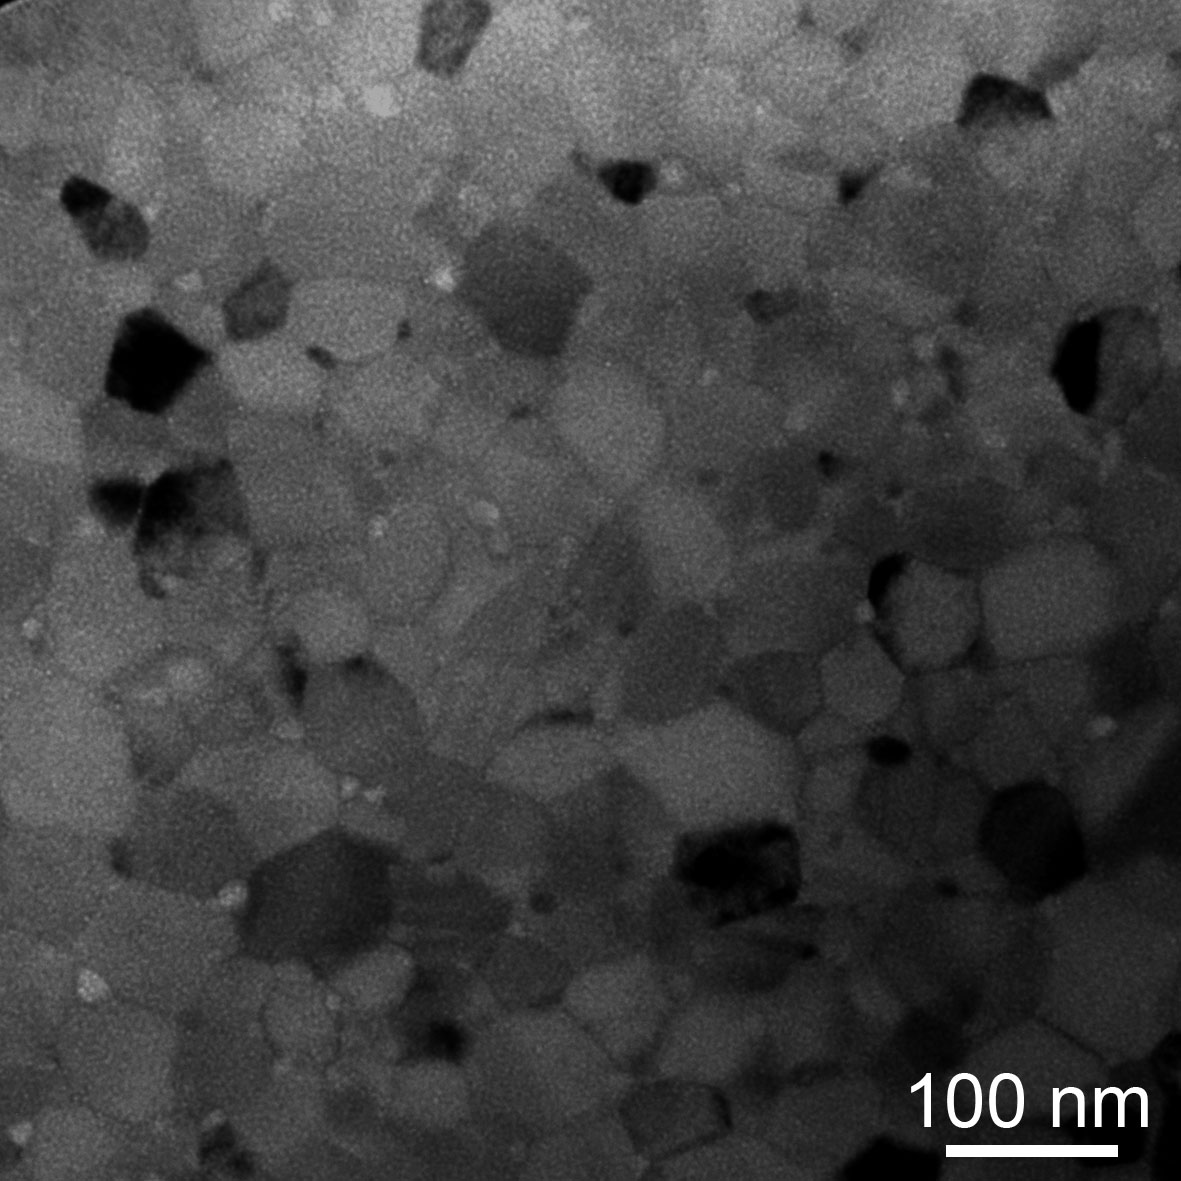
\includegraphics[scale=0.4]{img/TEM/Fig24c.jpg}} \qquad
					\subfloat[Muestra a $800 ^\circ C$]{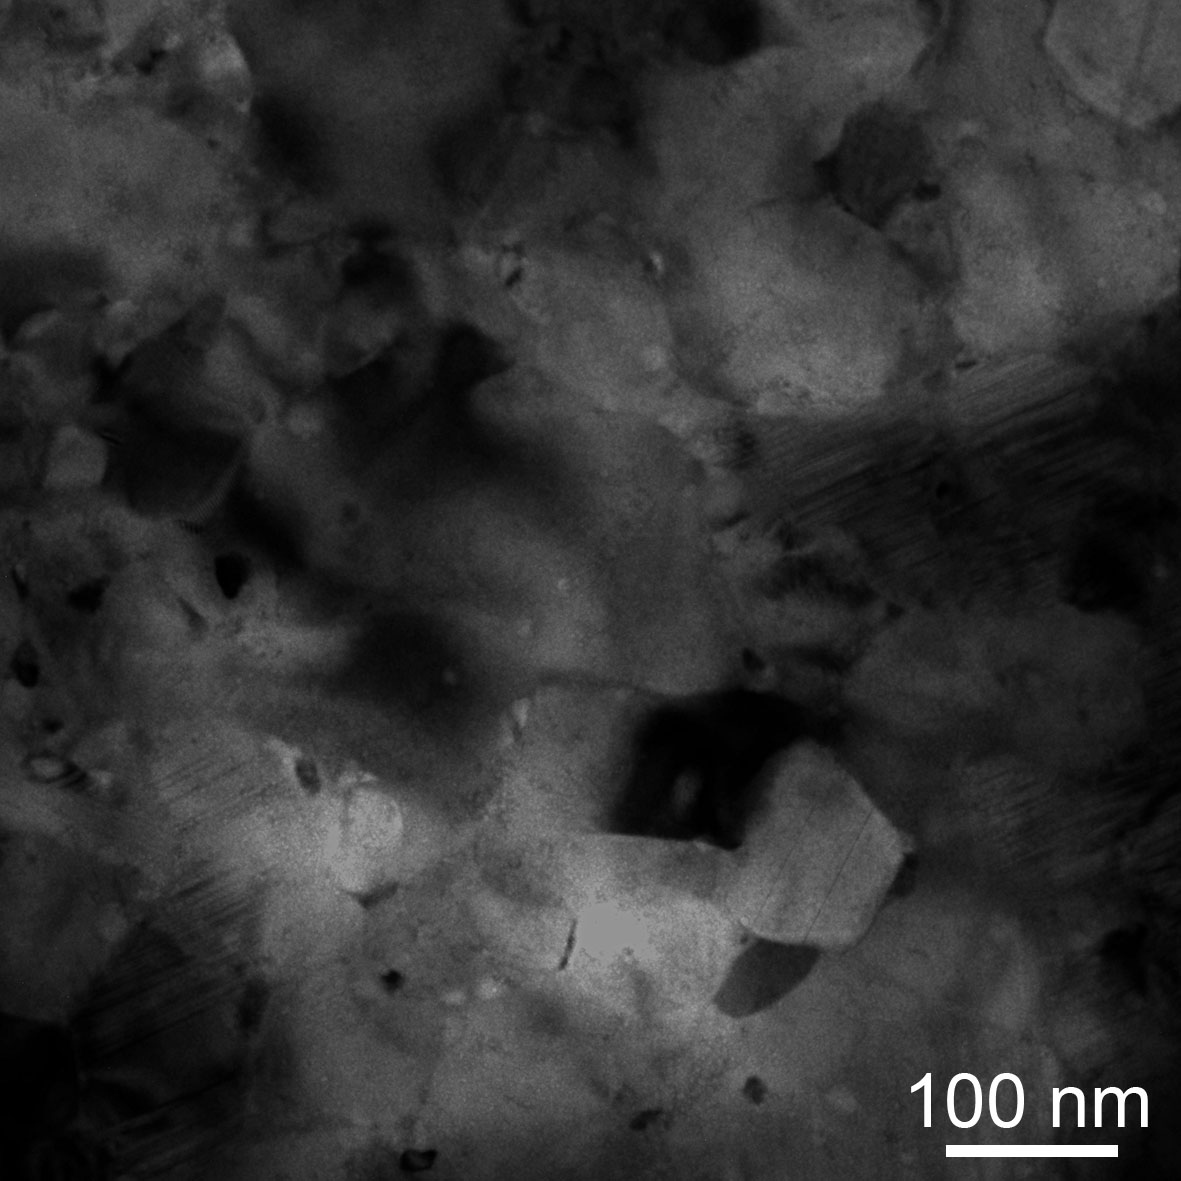
\includegraphics[scale=0.4]{img/TEM/Fig24d.jpg}}
					\caption*{Imágenes de TEM para las muestras pobres en $Ni$.}
				\end{figure}
			\end{frame}
			
			\begin{frame}
				\begin{table}[H]
					\centering
					\begin{tabular}{|c|c|c|}
					\hline
					\begin{tabular}[c]{@{}c@{}}Temperatura del\\ tratamiento $[^\circ C]$\end{tabular} & Fases halladas & Tamaño de grano {[}$nm${]} \\ \hline
					500 & B2 - $Ti_2Ni$                      & 10 a 50             \\ \hline
					600 & B2 - $Ti_2Ni$ - $NiZr$ - $\lambda$ & 110 a 140 - 10 a 30 \\ \hline
					700 & B2 - $Ti_2Ni$ - B19'               & $\sim$ 90           \\ \hline
					800 & B2 - $Ti_2Ni$ - $NiZr$               & 20 a 130            \\ \hline
					\end{tabular}
					\caption*{Fases halladas y tamaño de grano para cada tratamiento térmico en la deposición pobre en $Ni$.}
				\end{table}
			\end{frame}

		\subsubsection{Temperaturas de transformación}
			\begin{frame}{Curvas de DSC I}
				\begin{figure}[H]
				\captionsetup[subfloat]{labelformat=empty}
					\subfloat[Muestra tratada a $500 ^\circ C$]{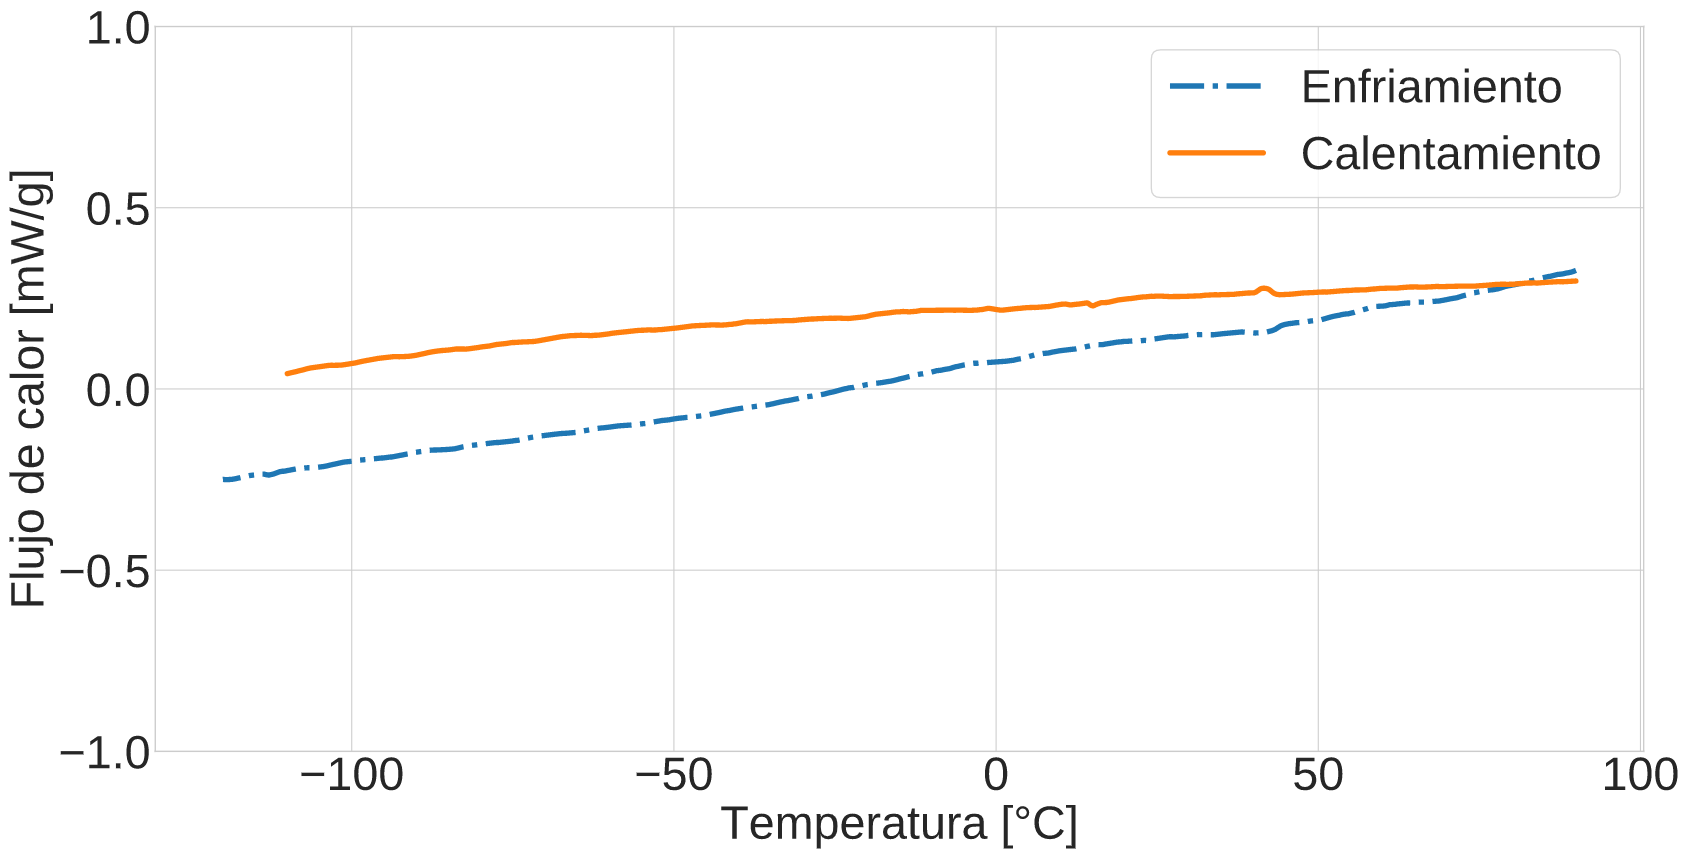
\includegraphics[scale=0.09]{img/DSCNiPoor/500}}
					\subfloat[Muestra tratada a $600 ^\circ C$]{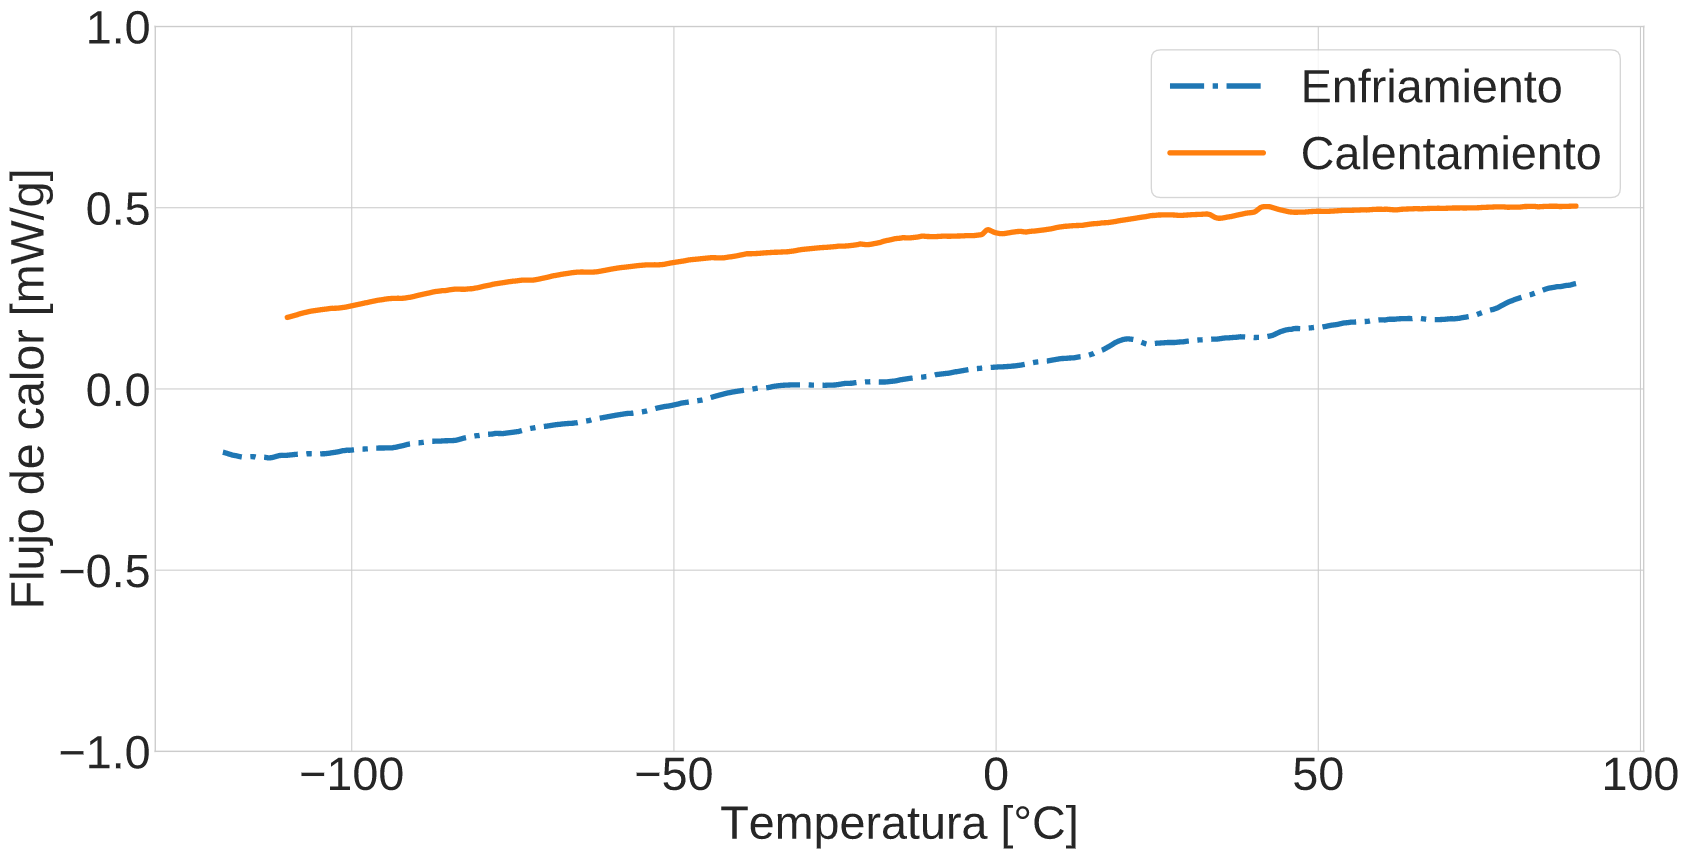
\includegraphics[scale=0.09]{img/DSCNiPoor/600}}
					\caption*{Curvas de DSC para las distintas muestras.}
				\end{figure}	
			\end{frame}
			
			\begin{frame}{Curvas de DSC II}
				\begin{figure}[H]
				\captionsetup[subfloat]{labelformat=empty}
					\subfloat[Muestra tratada a $700 ^\circ C$]{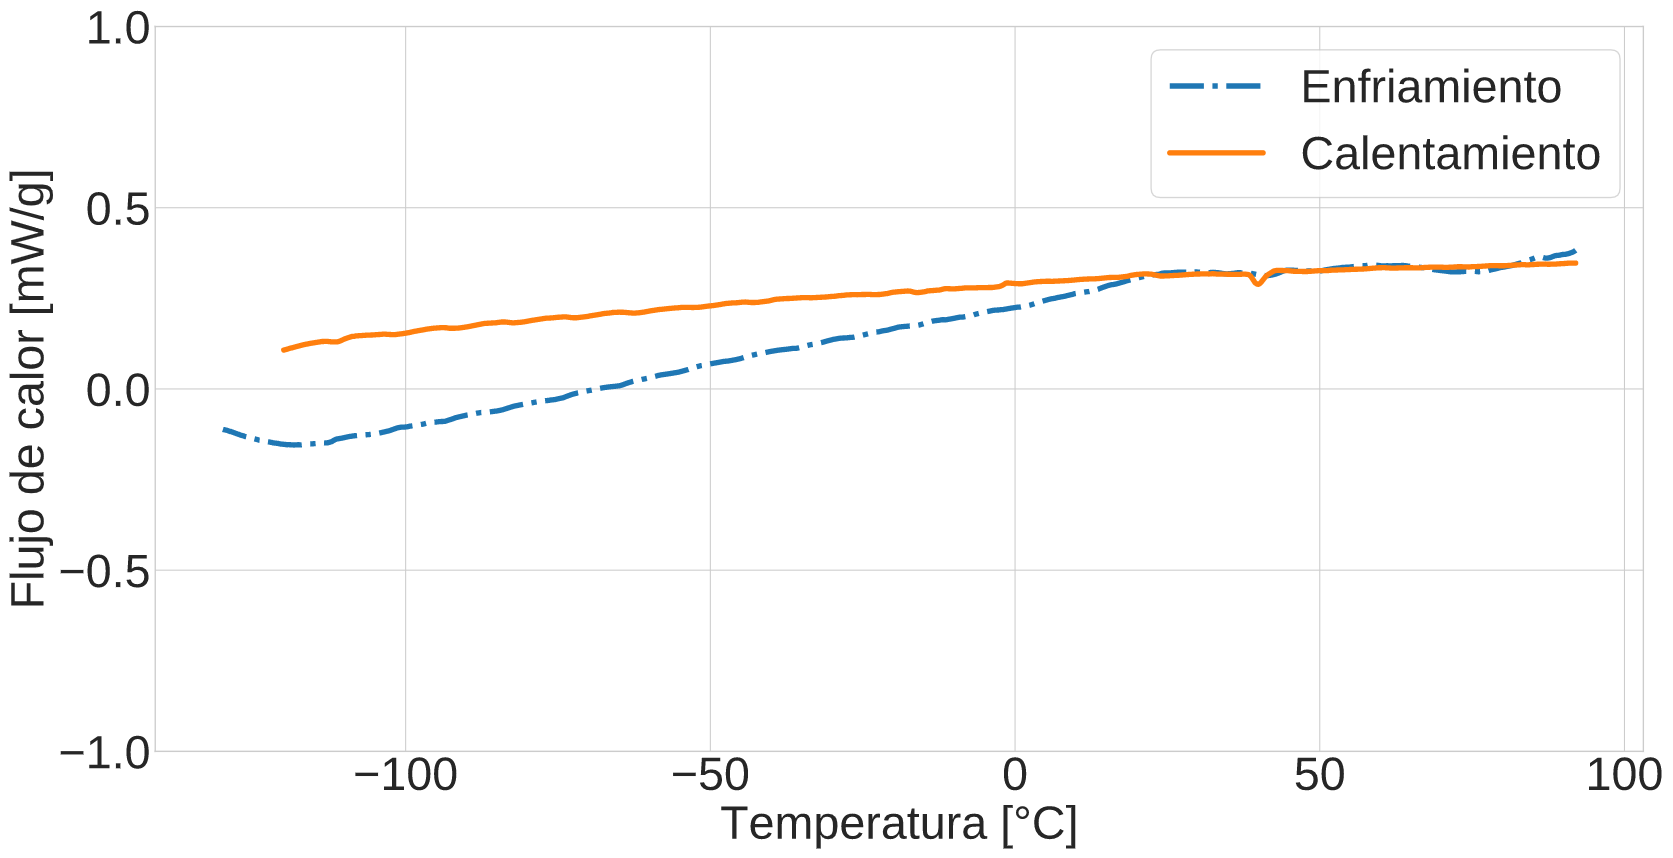
\includegraphics[scale=0.09]{img/DSCNiPoor/700}}
					\subfloat[Muestra tratada a $800 ^\circ C$]{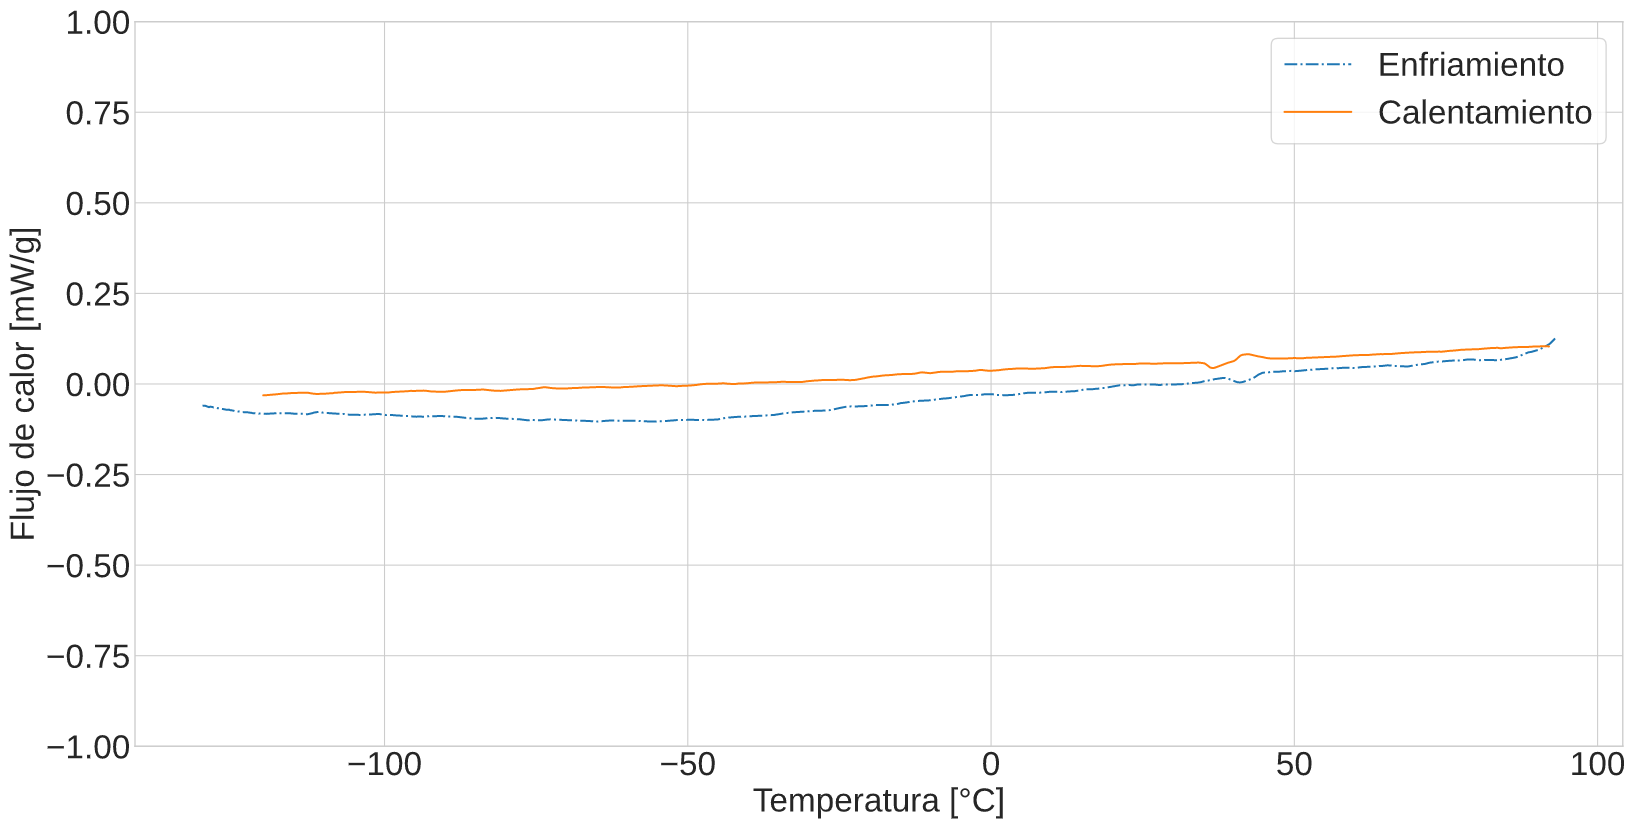
\includegraphics[scale=0.09]{img/DSCNiPoor/800}}
					\caption*{Curvas de DSC para las distintas muestras.}
				\end{figure}	
			\end{frame}
			
			\begin{frame}
				\begin{columns}
					\begin{column}{.49\textwidth}
						\begin{figure}
							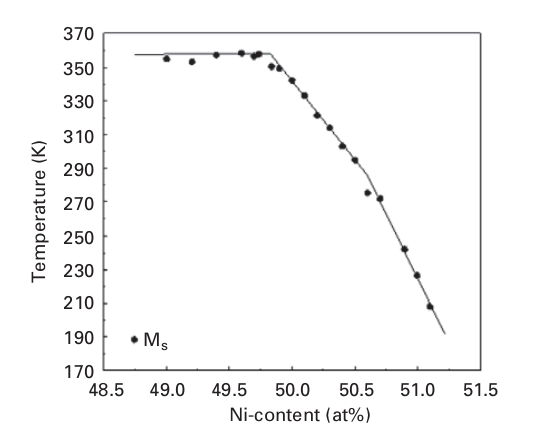
\includegraphics[scale=0.32]{img/MsNiDependence.png}
							\caption*{Efecto del porcentaje de Ni en la aleación NiTiZr.}
						\end{figure}
					\end{column}
					\begin{column}{.49\textwidth}
						\begin{figure}
							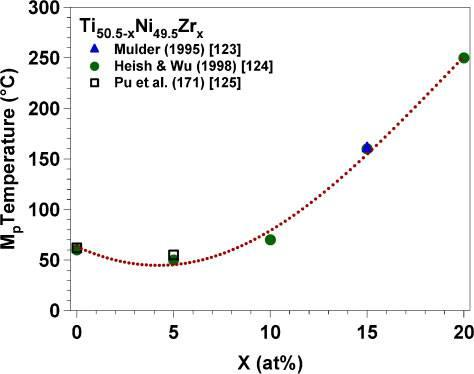
\includegraphics[scale=0.32]{img/MsZrDependence.jpeg}
							\caption*{Efecto del porcentaje de Zr en la aleación NiTiZr.}				
						\end{figure}
					\end{column}
				\end{columns}
			\end{frame}
			
	\subsection{Ricas en $Ni$}	
		\subsubsection{Fases obtenidas}
			\begin{frame}{Difracción por rayos X I}
				\begin{figure}[H]
				\captionsetup[subfloat]{labelformat=empty}
					\subfloat[Muestra a $500 ^\circ C$]{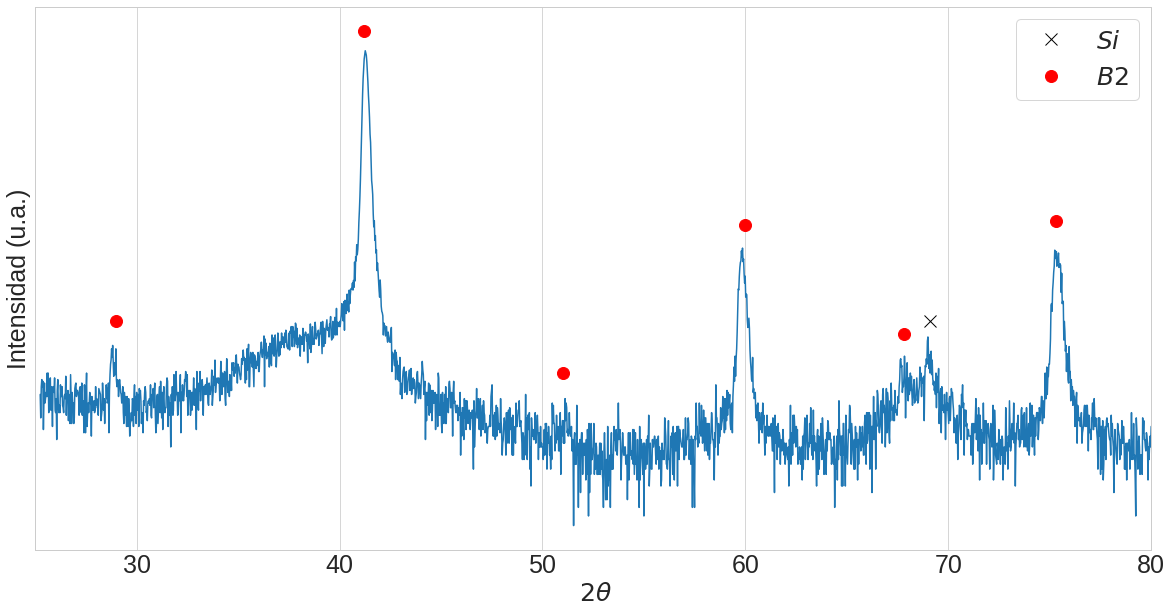
\includegraphics[scale=0.12]{img/RX/NiRich_500.png}} \qquad
					\subfloat[Muestra a $600 ^\circ C$]{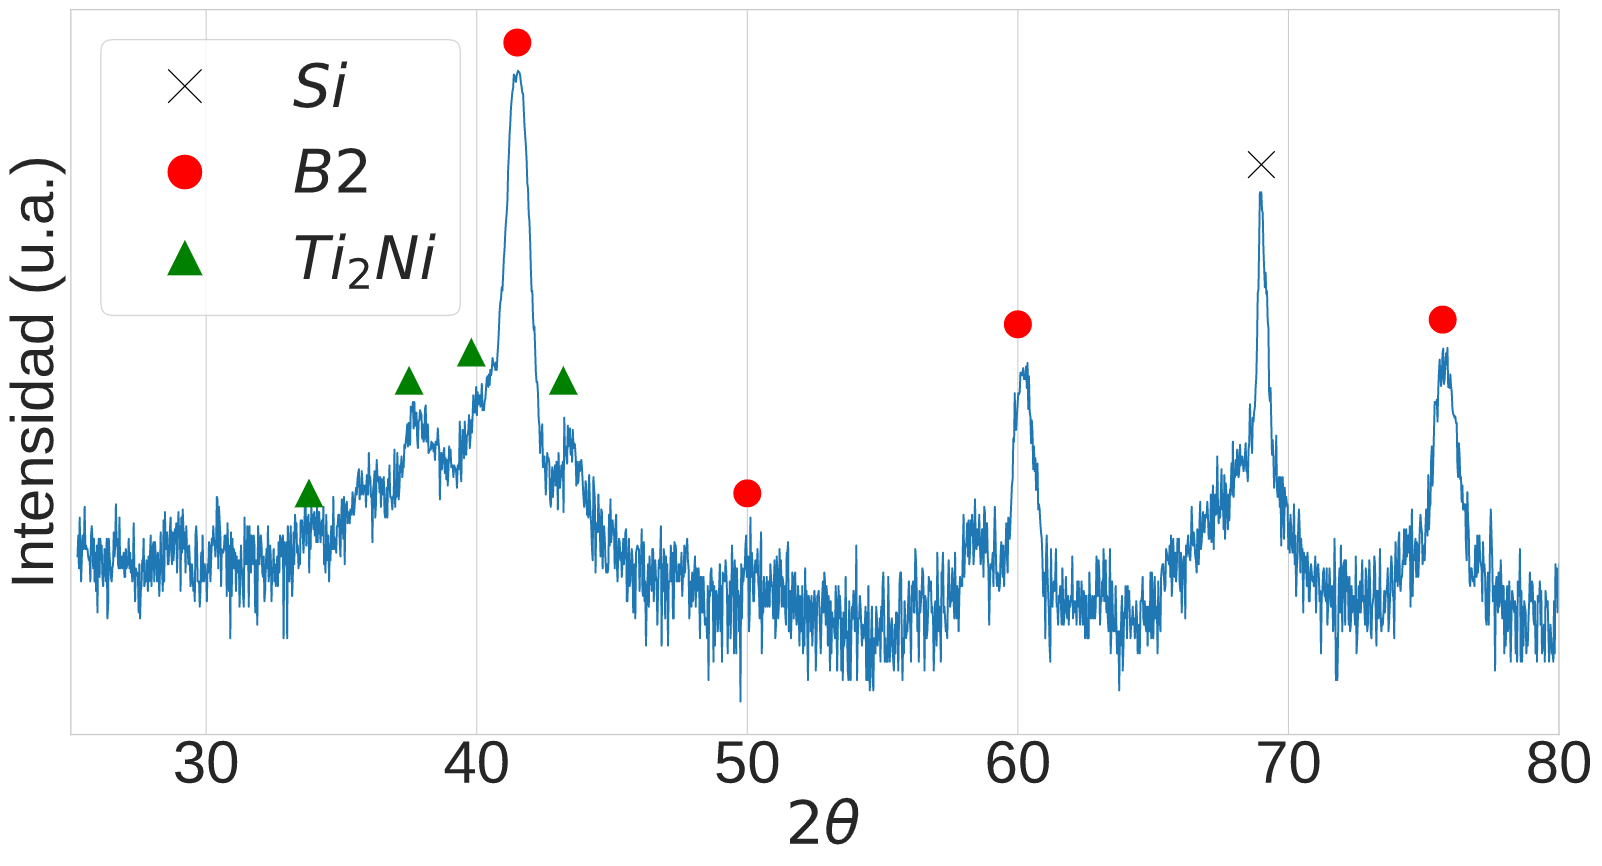
\includegraphics[scale=0.12]{img/RX/NiRich_600.png}}
					\caption*{Patrones de difracción para las muestras pobres en $Ni$.}
				\end{figure}		
			\end{frame}
			
			\begin{frame}{Difracción por rayos X II}
				\begin{figure}[H]
				\captionsetup[subfloat]{labelformat=empty}
					\subfloat[Muestra a $700 ^\circ C$]{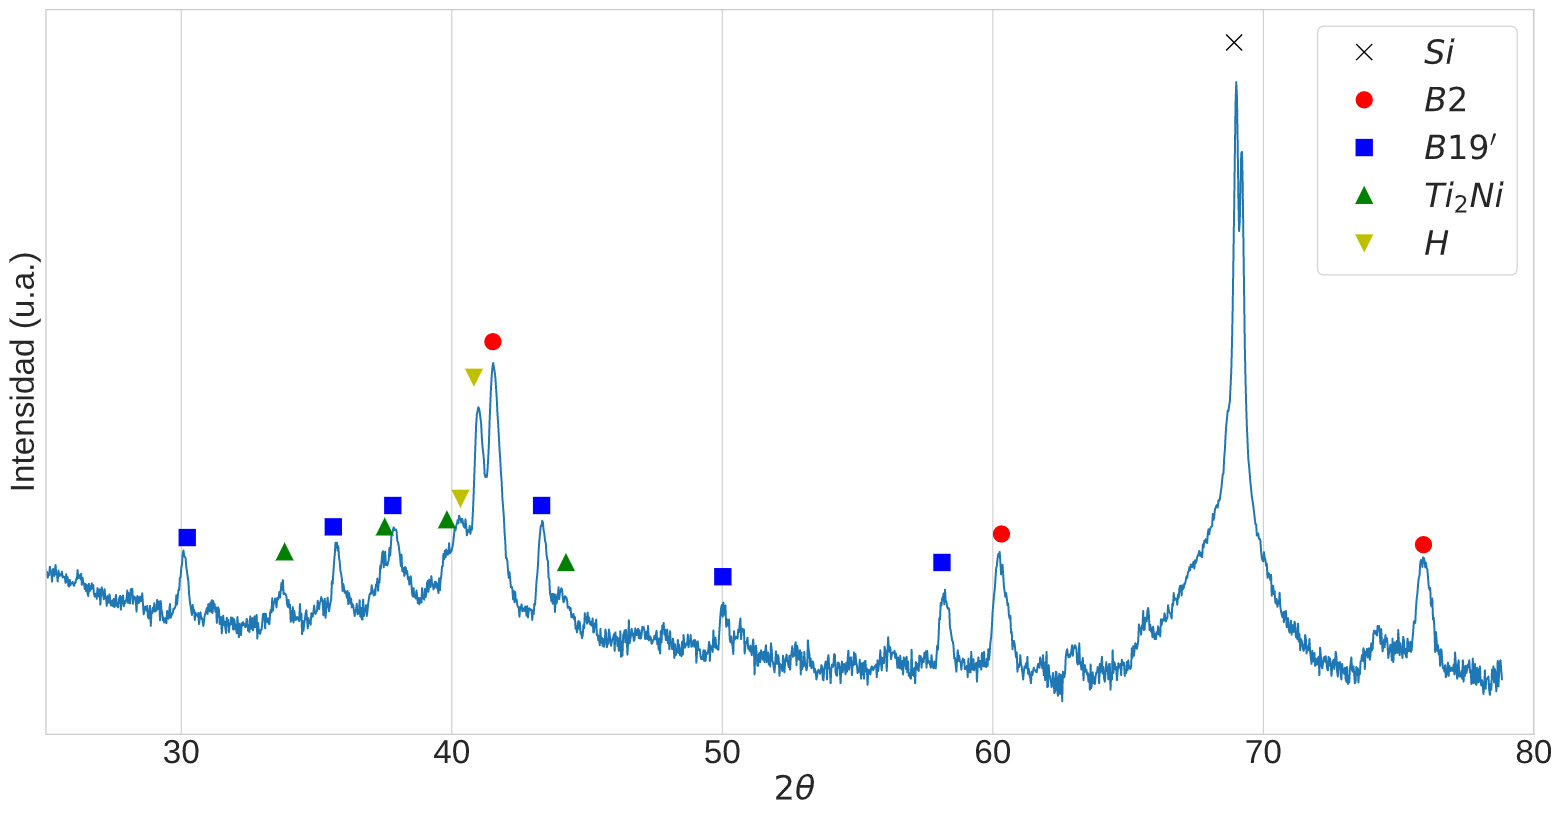
\includegraphics[scale=0.0912]{img/RX/NiRich_700.png}} \qquad
					\subfloat[Muestra a $800 ^\circ C$]{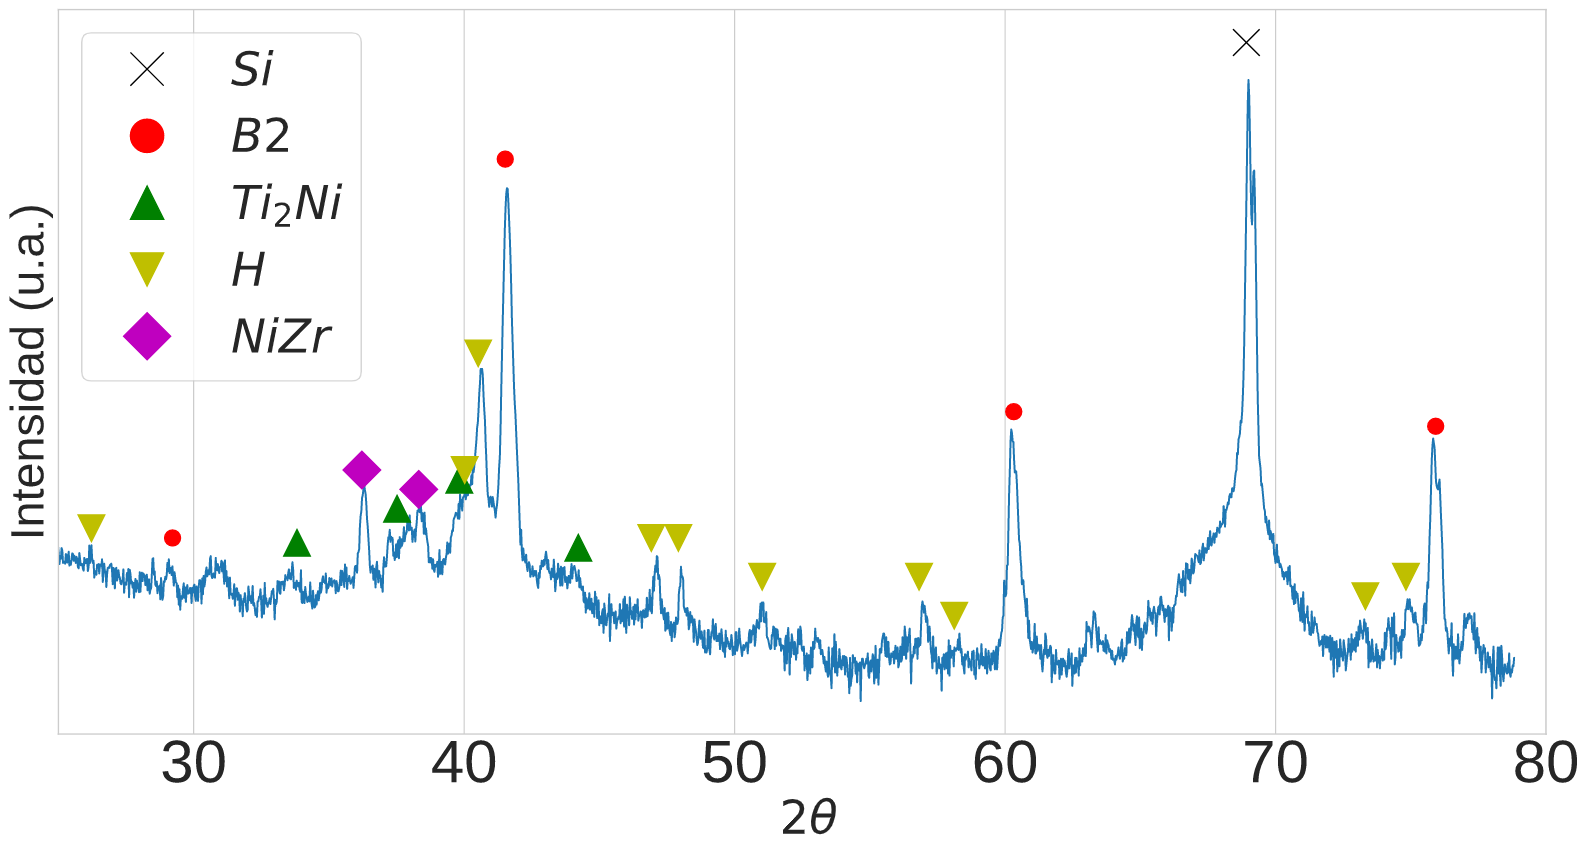
\includegraphics[scale=0.12]{img/RX/NiRich_800.png}} \\
					\caption*{Patrones de difracción para las muestras pobres en $Ni$.}
				\end{figure}		
			\end{frame}
	
			\begin{frame}{Imágenes obtenidas por TEM I}
				 \begin{figure}[H]
				 	\captionsetup[subfloat]{labelformat=empty}
					\centering
					\subfloat[Muestra a $500 ^\circ C$]{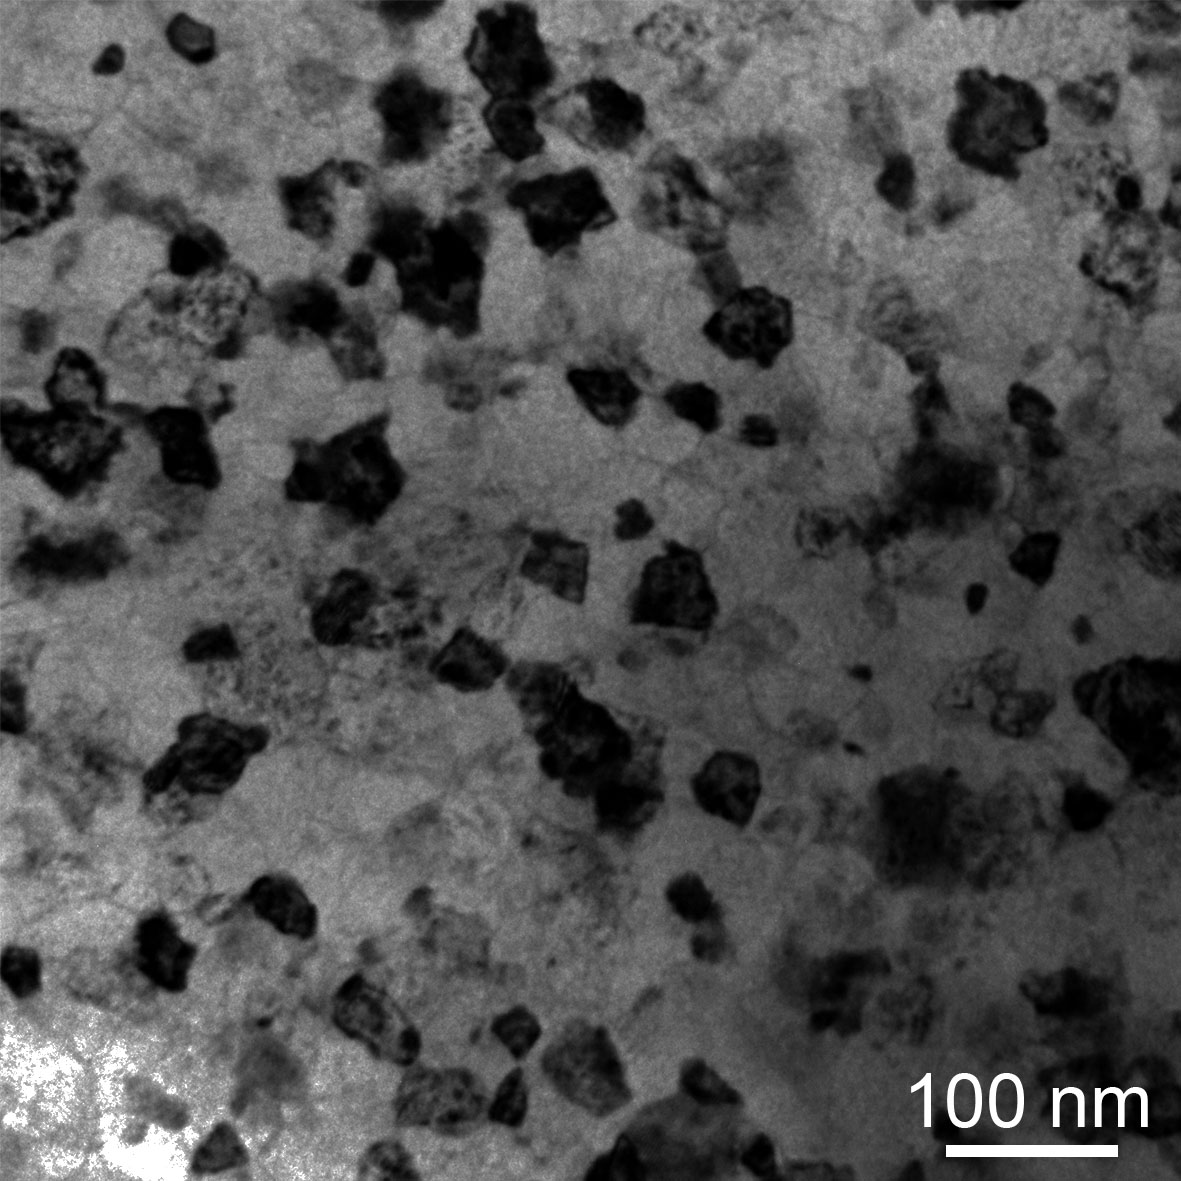
\includegraphics[scale=0.4]{img/TEM/Fig27a.jpg}} \qquad
					\subfloat[Muestra a $600 ^\circ C$]{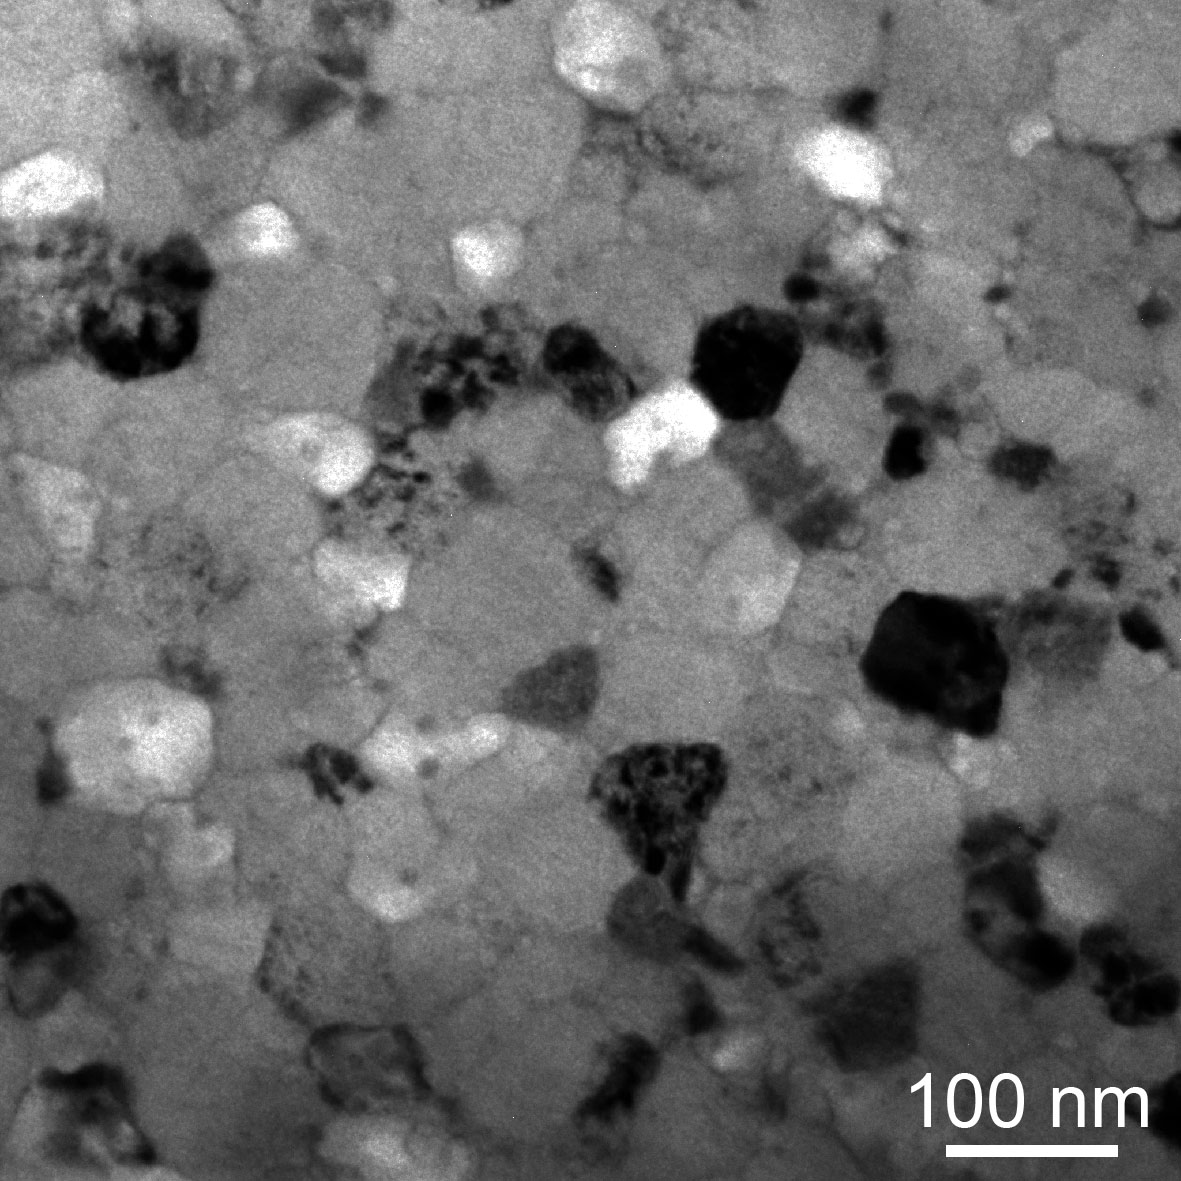
\includegraphics[scale=0.4]{img/TEM/Fig27b.jpg}}
					\caption*{Imágenes de TEM para las muestras ricas en $Ni$.}
					\label{TEMNiRich}
				\end{figure}
			\end{frame}
			\begin{frame}{Imágenes obtenidas por TEM II}
				 \begin{figure}[H]
				 	\captionsetup[subfloat]{labelformat=empty}
					\centering
					\subfloat[Muestra a $700 ^\circ C$]{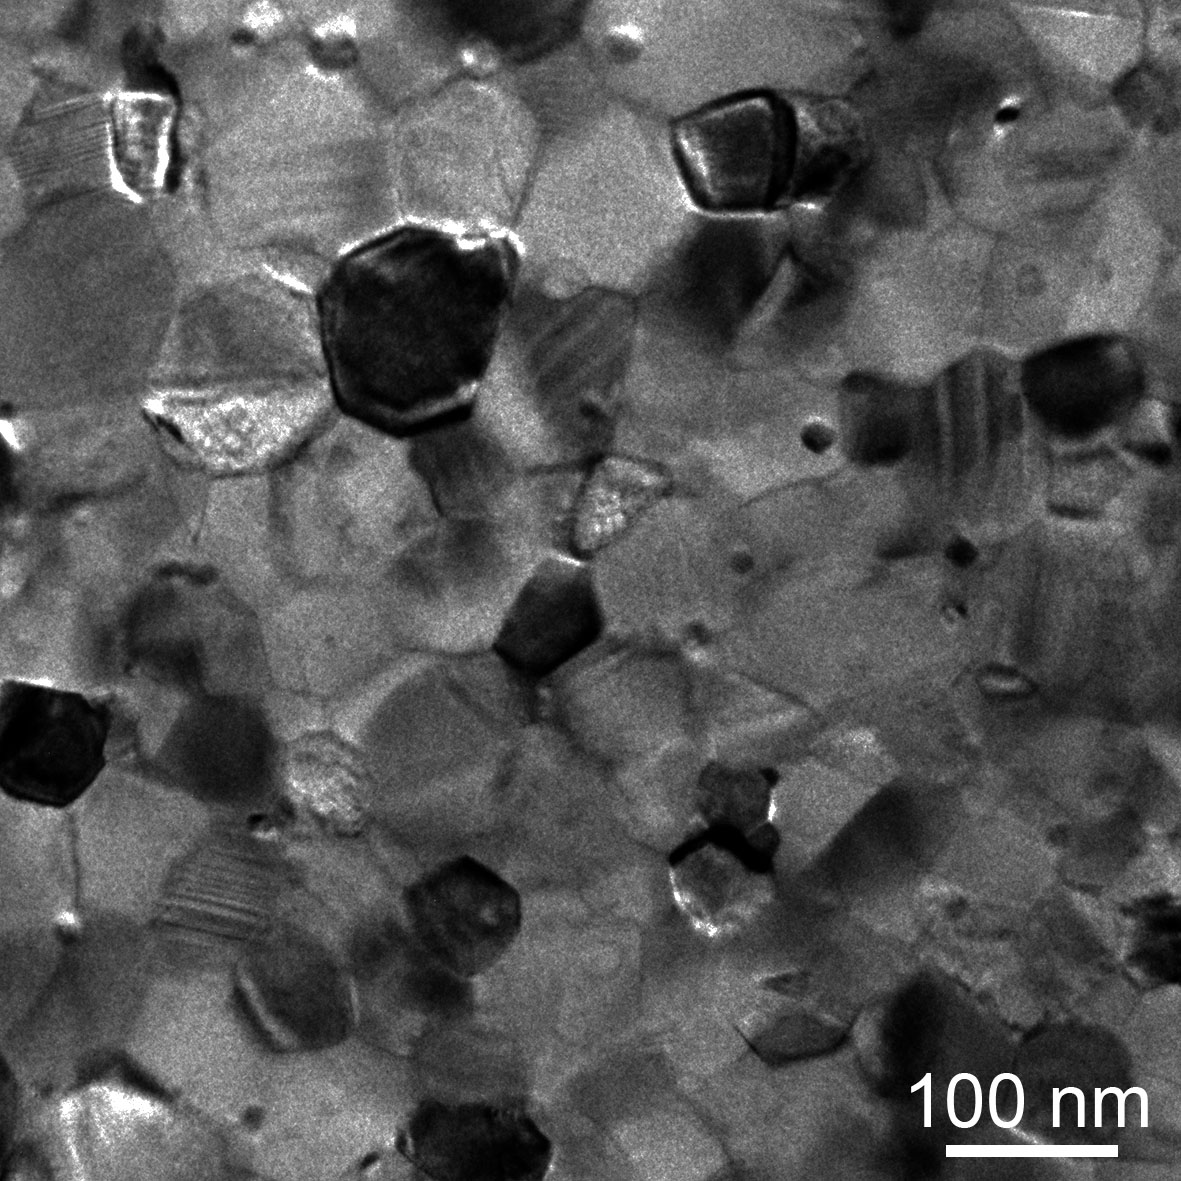
\includegraphics[scale=0.4]{img/TEM/Fig27c.jpg}}	\qquad
					\subfloat[Muestra a $800 ^\circ C$]{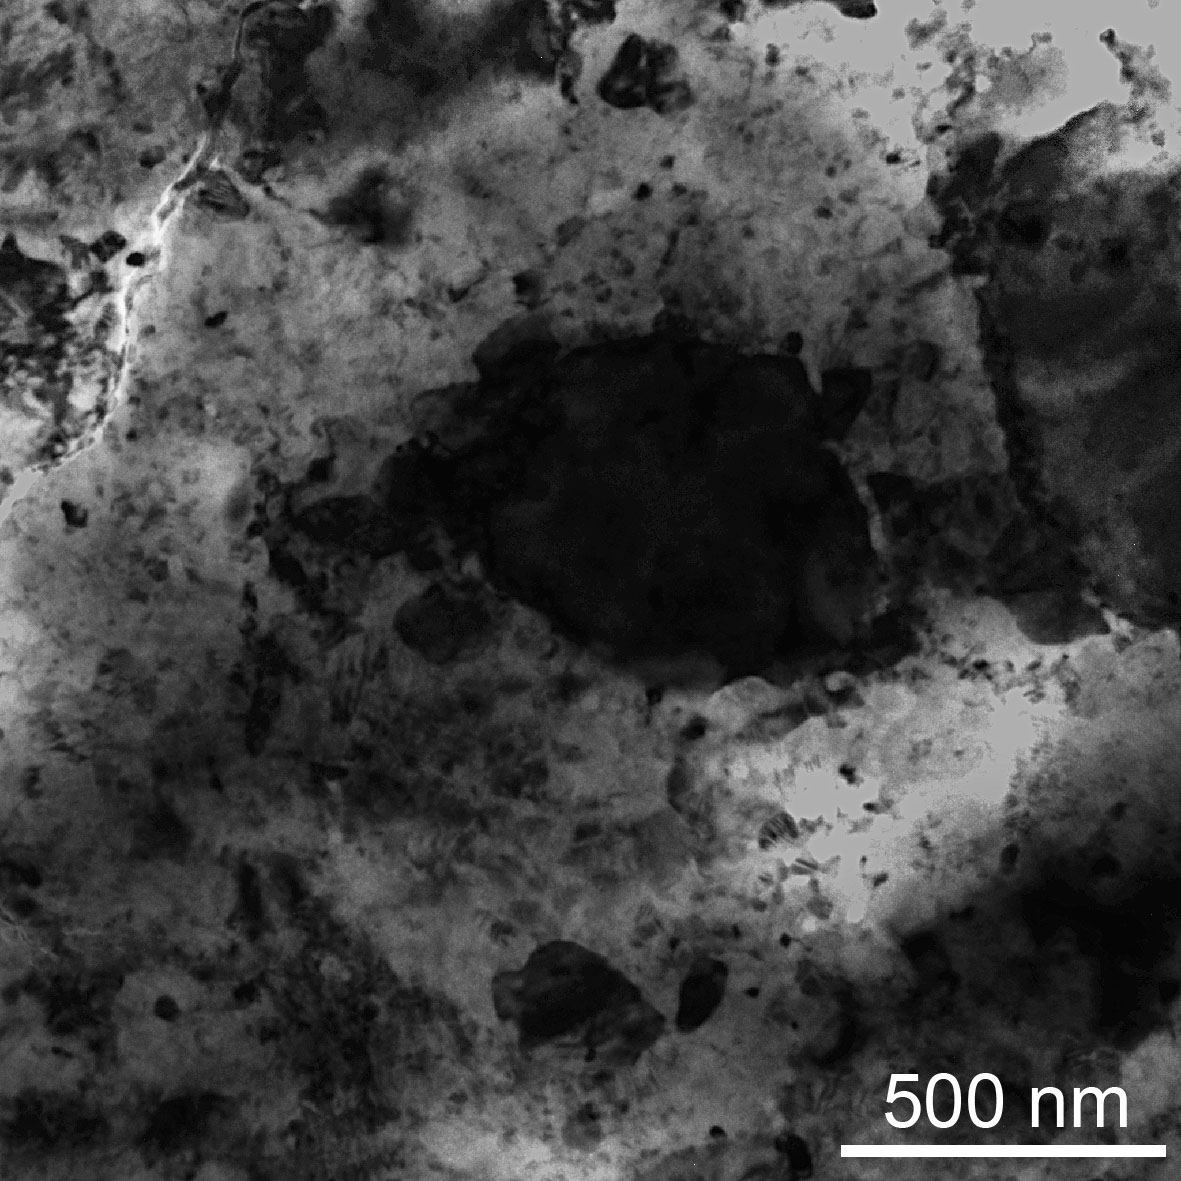
\includegraphics[scale=0.4]{img/TEM/Fig27d.jpg}}
					\caption*{Imágenes de TEM para las muestras ricas en $Ni$.}
					\label{TEMNiRich}
				\end{figure}
			\end{frame}
			
			\begin{frame}{Fases obtenidas}
				\begin{table}[H]
					\centering
					\begin{tabular}{|c|c|c|}
					\hline
					\begin{tabular}[c]{@{}c@{}}Temperatura del\\ tratamiento $[^\circ C]$\end{tabular} & Fases halladas & Tamaño de grano {[}$nm${]} \\ \hline
					500 & B2                         & $\sim$ 70  \\ \hline
					600 & B2 - $Ti_2Ni$              & $\sim$ 90  \\ \hline
					700 & B2 - $Ti_2Ni$ - B19' - H   & $\sim$ 115 \\ \hline
					800 & B2 - $Ti_2Ni$ - H - $NiZr$ & 50 a 500      \\ \hline
					\end{tabular}
					\caption*{Fases halladas para cada tratamiento térmico en la deposición rica en $Ni$.}
				\end{table}
			\end{frame}
		\subsubsection{Temperaturas de transformación}
			\begin{frame}
				\begin{figure}[H]
					\captionsetup[subfloat]{labelformat=empty}
					\noindent\makebox[\linewidth][c]{
						\subfloat[Muestra tratada a $500 ^\circ C$]{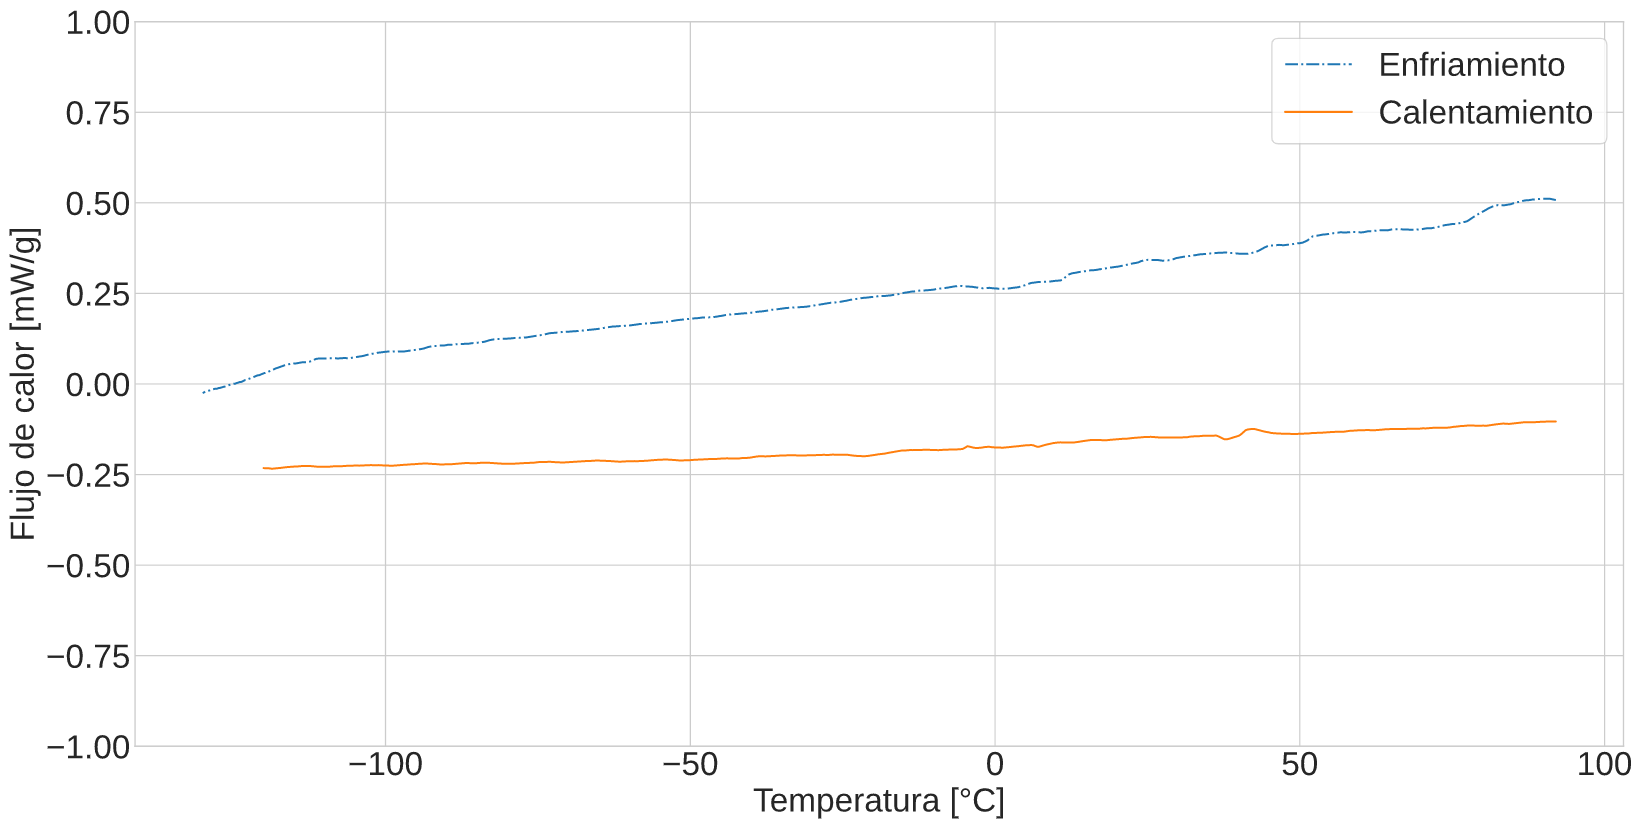
\includegraphics[scale=0.08]{img/DSCNiRich/500NiRich}}
						\subfloat[Muestra tratada a $600 ^\circ C$]{\includegraphics[scale=0.08]{img/DSCNiRich/600NiRich}}}\\
						
					\noindent\makebox[\linewidth][c]{
					\subfloat[Muestra tratada a $700 ^\circ C$]
					{\includegraphics[scale=0.08]{img/DSCNiRich/700NiRich}}}
					 \caption*{Curvas de DSC para muestras ricas en $Ni$ tratadas a diferentes temperaturas.}	
				\end{figure}		
			\end{frame}
		
			\begin{frame}[allowframebreaks]{Curvas de Resistividad}
				\begin{figure}[H]
				\captionsetup[subfloat]{labelformat=empty}
					\centering
					\subfloat[Muestra a $500 ^\circ C$]{\includegraphics[scale=0.08]{img/Resistance_500_alt.png}} \qquad
					\subfloat[Muestra a $600 ^\circ C$]{\includegraphics[scale=0.08]{img/Resistance_600_alt.png}}\\
					\subfloat[Muestra a $800 ^\circ C$]{\includegraphics[scale=0.08]{img/Resistance_800_alt.png}} 
					\caption*{Mediciones del método de resistividad de cuatro puntas en las cuales no fue posible hallar las temperaturas de transformación.}
				\end{figure}
			\end{frame}
				
			\begin{frame}
				\begin{figure}[H]
					\centering
					\includegraphics[scale=0.2]{img/Resistance_700.png}
					\caption*{Curva medida por el método de resistividad de cuatro puntas para la muestra tratada a 700$^\circ C$.}
				\end{figure}
			\end{frame}
	

\section{Conclusión}
	\begin{frame}[allowframebreaks]{Conclusiones}
		\begin{itemize}
			\item Se obtuvieron 12 láminas delgadas de aproximadamente 8 mm x 25 mm c/u.
			\item Una deposición rica en Ni (50,4 at\% $Ni$, 30,8 at\% $Ti$ y 18,9 at\% $Zr$) y otra pobre en Ni(46 at\% $Ni$, 33,2 at\% $Ti$ y 20,8 at\% $Zr$).
			\item Por el método de Kissinger se obtuvo una energía de activación de (420 $\pm$ 30) $kJ$ y por el de Augis-Bennet de (410 $\pm$ 30) $kJ$, ambos valores coincidentes entre sí y comparables con los informados por otros autores.
			\item Las muestras de ambas deposiciones fueron tratadas termicamente por una hora en atmósfera de $Ar$ a 3 $mTorr$ a $500^\circ C$, $600^\circ C$, $700^\circ C$ y $800^\circ C$.
			\item Mediante TEM y RX se hallaron para las muestras pobres en $Ni$ las fases B2, $(Ti, Zr)_2Ni$ (o posiblemente $(Ti, Zr)_4Ni_2O$), $\lambda$ y $NiZr$.
			\item Para las muestras ricas en $Ni$, adicionalmente, se halló la fase H, pero no la fase $\lambda$.
			\item Mediante DSC en ninguna muestra pudo ser detectada una transformación de fase.
			\item Mediante resistividad por el método de cuatro puntas, se determinaron las temperaturas de transformación para la muestra rica en $Ni$ tratada a $700^\circ C$.
			\item Los motivos por los cuales las temperaturas de transformación fueron más bajas de lo esperado fueron por la presencia de fases adicionales que removían $Zr$ y $Ti$ de la fase matriz, sumado al bajo tamaño de grano, que requería un sobreenfriamiento mayor.
		\end{itemize}
	\end{frame}
	
	\begin{frame}{Perspectivas a futuro}
En base a lo visto en este trabajo, se propone en futuros estudios la optimización de los tratamientos térmicos para seleccionar la microestructura con precipitados nanométricos en el interior de los granos de la fase matriz, de modo de endurecerla sin cambiar drásticamente su estequiometría. Se sugiere, en particular, continuar con el estudio de las láminas ricas en $Ni$, ya que está demostrado la eficiencia de la fase H para endurecer la fase matriz en las aleaciones producidas por métodos convencionales, sin embargo no hay estudios en láminas delgadas de dicha composición en la bibliografía.	
\end{frame}
\end{document}
%		\begin{frame}{Difracción por RX}
%		\begin{columns}
%		\begin{column}{.49\textwidth}
%		\end{column}
%		\begin{column}{.49\textwidth}
%		\end{column}
%		\end{columns}
